
%%%%%%%%%%%%%%%%%%%%%%%%%%%%%%%%%%%%%%%%%%%%%%%%%%%%%%%%%%%%%%%%%%%%%
%% This is a (brief) model paper using the achemso class
%% The document class accepts keyval options, which should include
%% the target journal and optionally the manuscript type. 
%%%%%%%%%%%%%%%%%%%%%%%%%%%%%%%%%%%%%%%%%%%%%%%%%%%%%%%%%%%%%%%%%%%%%
\documentclass[journal=jacsat,manuscript=article]{achemso}

%%%%%%%%%%%%%%%%%%%%%%%%%%%%%%%%%%%%%%%%%%%%%%%%%%%%%%%%%%%%%%%%%%%%%
%% Place any additional packages needed here.  Only include packages
%% which are essential, to avoid problems later. Do NOT use any
%% packages which require e-TeX (for example etoolbox): the e-TeX
%% extensions are not currently available on the ACS conversion
%% servers.
%%%%%%%%%%%%%%%%%%%%%%%%%%%%%%%%%%%%%%%%%%%%%%%%%%%%%%%%%%%%%%%%%%%%%
\usepackage[version=3]{mhchem} % Formula subscripts using \ce{}
\usepackage{siunitx}
\usepackage{tabularx}
\usepackage{float}
\usepackage{booktabs}

\usepackage{amsmath}
\usepackage{amssymb}
\usepackage{amsfonts}
\usepackage{graphicx}
\DeclareMathOperator*{\argmax}{arg\,max}
\DeclareMathOperator*{\argmin}{arg\,min}
\newcommand{\SIci}[4]{\SI{#1}{#4},\ \SI{95}{\percent}C.I.\ [\numrange[range-phrase=---]{#2}{#3} \si{#4}]}
\newcommand{\numci}[3]{\num{#1},\ \SI{95}{\percent}C.I.\ [\numrange[range-phrase=---]{#2}{#3}]}

%%%%%%%%%%%%%%%%%%%%%%%%%%%%%%%%%%%%%%%%%%%%%%%%%%%%%%%%%%%%%%%%%%%%%
% supplementary materials
\usepackage{xr}
\newcommand*\sref[1]{%
    S\ref{#1}}
    
\makeatletter
\newcommand*{\addFileDependency}[1]{% argument=file name and extension
  \typeout{(#1)}
  \@addtofilelist{#1}
  \IfFileExists{#1}{}{\typeout{No file #1.}}
}
\makeatother

\newcommand*{\myexternaldocument}[1]{%
    \externaldocument{#1}%
    \addFileDependency{#1.tex}%
    \addFileDependency{#1.aux}%
    }
    
\myexternaldocument{SI}
%%%%%%%%%%%%%%%%%%%%%%%%%%%%%%%%%%%%%%%%%%%%%%%%%%%%%%%%%%%%%%%%%%%%%

% \usepackage{caption}
% \captionsetup[table]{position=bottom} 
% \usepackage{subcaption}
% \usepackage{bm} % e.g., \bm(\mu)
% \usepackage{xfrac}  % e.g., \sfrac{1}{2}                   
% \usepackage{relsize} % e.g., \mathlarger 
% \usepackage{algorithm2e}
% \DeclareMathOperator*{\argmax}{arg\,max}
% \DeclareMathOperator*{\argmin}{arg\,min}

%%%%%%%%%%%%%%%%%%%%%%%%%%%%%%%%%%%%%%%%%%%%%%%%%%%%%%%%%%%%%%%%%%%%%
%% If issues arise when submitting your manuscript, you may want to
%% un-comment the next line.  This provides information on the
%% version of every file you have used.
%%%%%%%%%%%%%%%%%%%%%%%%%%%%%%%%%%%%%%%%%%%%%%%%%%%%%%%%%%%%%%%%%%%%%
%%\listfiles

%%%%%%%%%%%%%%%%%%%%%%%%%%%%%%%%%%%%%%%%%%%%%%%%%%%%%%%%%%%%%%%%%%%%%
%% Place any additional macros here.  Please use \newcommand* where
%% possible, and avoid layout-changing macros (which are not used
%% when typesetting).
%%%%%%%%%%%%%%%%%%%%%%%%%%%%%%%%%%%%%%%%%%%%%%%%%%%%%%%%%%%%%%%%%%%%%
\newcommand*\mycommand[1]{\texttt{\emph{#1}}}

%%%%%%%%%%%%%%%%%%%%%%%%%%%%%%%%%%%%%%%%%%%%%%%%%%%%%%%%%%%%%%%%%%%%%
%% Meta-data block
%% ---------------
%% Each author should be given as a separate \author command.
%%
%% Corresponding authors should have an e-mail given after the author
%% name as an \email command. Phone and fax numbers can be given
%% using \phone and \fax, respectively; this information is optional.
%%
%% The affiliation of authors is given after the authors; each
%% \affiliation command applies to all preceding authors not already
%% assigned an affiliation.
%%
%% The affiliation takes an option argument for the short name.  This
%% will typically be something like "University of Somewhere".
%%
%% The \altaffiliation macro should be used for new address, etc.
%% On the other hand, \alsoaffiliation is used on a per author basis
%% when authors are associated with multiple institutions.
%%%%%%%%%%%%%%%%%%%%%%%%%%%%%%%%%%%%%%%%%%%%%%%%%%%%%%%%%%%%%%%%%%%%%

\author{Robert E. Arbon}
\altaffiliation{ReDesign Science, New York, NY, USA}
\author{Antonia S.J.S. Mey}
\email{antonia.mey@ed.ac.uk}
\affiliation[Unknown University]
{EaStCHEM School of Chemistry, David Brewster Road, Joseph Black Building, The King’s Buildings, Edinburgh, EH93FJ, UK}

%%%%%%%%%%%%%%%%%%%%%%%%%%%%%%%%%%%%%%%%%%%%%%%%%%%%%%%%%%%%%%%%%%%%%
%% The document title should be given as usual. Some journals require
%% a running title from the author: this should be supplied as an
%% optional argument to \title.
%%%%%%%%%%%%%%%%%%%%%%%%%%%%%%%%%%%%%%%%%%%%%%%%%%%%%%%%%%%%%%%%%%%%%
\title[]{Sensitivity test of Markov state models}

%%%%%%%%%%%%%%%%%%%%%%%%%%%%%%%%%%%%%%%%%%%%%%%%%%%%%%%%%%%%%%%%%%%%%
%% Some journals require a list of abbreviations or keywords to be
%% supplied. These should be set up here, and will be printed after
%% the title and author information, if needed.
%%%%%%%%%%%%%%%%%%%%%%%%%%%%%%%%%%%%%%%%%%%%%%%%%%%%%%%%%%%%%%%%%%%%%
\abbreviations{IR,NMR,UV}
\keywords{American Chemical Society, \LaTeX}

%%%%%%%%%%%%%%%%%%%%%%%%%%%%%%%%%%%%%%%%%%%%%%%%%%%%%%%%%%%%%%%%%%%%%
%% The manuscript does not need to include \maketitle, which is
%% executed automatically.
%%%%%%%%%%%%%%%%%%%%%%%%%%%%%%%%%%%%%%%%%%%%%%%%%%%%%%%%%%%%%%%%%%%%%
\begin{document}

%%%%%%%%%%%%%%%%%%%%%%%%%%%%%%%%%%%%%%%%%%%%%%%%%%%%%%%%%%%%%%%%%%%%%
%% The "tocentry" environment can be used to create an entry for the
%% graphical table of contents. It is given here as some journals
%% require that it is printed as part of the abstract page. It will
%% be automatically moved as appropriate.
%%%%%%%%%%%%%%%%%%%%%%%%%%%%%%%%%%%%%%%%%%%%%%%%%%%%%%%%%%%%%%%%%%%%%
\begin{tocentry}

Some journals require a graphical entry for the Table of Contents.
This should be laid out ``print ready'' so that the sizing of the
text is correct.

Inside the \texttt{tocentry} environment, the font used is Helvetica
8\,pt, as required by \emph{Journal of the American Chemical
Society}.

The surrounding frame is 9\,cm by 3.5\,cm, which is the maximum
permitted for  \emph{Journal of the American Chemical Society}
graphical table of content entries. The box will not resize if the
content is too big: instead it will overflow the edge of the box.

This box and the associated title will always be printed on a
separate page at the end of the document.

\end{tocentry}

%%%%%%%%%%%%%%%%%%%%%%%%%%%%%%%%%%%%%%%%%%%%%%%%%%%%%%%%%%%%%%%%%%%%%
%% The abstract environment will automatically gobble the contents
%% if an abstract is not used by the target journal.
%%%%%%%%%%%%%%%%%%%%%%%%%%%%%%%%%%%%%%%%%%%%%%%%%%%%%%%%%%%%%%%%%%%%%
\begin{abstract}
  Abstract
\end{abstract}

%%%%%%%%%%%%%%%%%%%%%%%%%%%%%%%%%%%%%%%%%%%%%%%%%%%%%%%%%%%%%%%%%%%%%
%% Start the main part of the manuscript here.
%%%%%%%%%%%%%%%%%%%%%%%%%%%%%%%%%%%%%%%%%%%%%%%%%%%%%%%%%%%%%%%%%%%%%
\section{Introduction}
Introduction



Do VAMP scores matter?  Compare low scoring with high scoring

\section{Theory}
\subsection{Markov state models}
\subsection{Gaussian processes}

\section{Methods}
\subsection{Molecular dynamics}

This work used eight of the twelve fast-folding proteins which have become the de-facto benchmark dataset for testing molecular kinetics methods. The methods used to create this data are described elsewhere. The proteins used, their PDB accession codes, the amount of simulation data, the number of residues and the average folding timescale are shown in table \ref{tab:data_description}. Each long trajectory was split into sub-trajectories of length \SI{200}{\nano\second}. 

\begin{table}
    \caption{\textsc{Description of molecular dynamics data}}
    \begin{tabularx}{\textwidth}{llXXXX}
    \toprule
    Name & PDB & Simulation time (\si{\micro\second}) & Average folding time (\si{\micro\second}) & No. Residues & \\
    \midrule
    Chignolin           & cln025    & \num{106}     & \num{0.6} & 10 & \\
    Trp-cage            & 2JOF      & \num{208}     & \num{14}  & 20 & \\
    BBA                 & 1FME      & \num{325}     & \num{18}  & 28 & \\
    Villin              & 2F4K      & \num{125}     & \num{2.8} & 35  &\\
    WW domain           & 2F21      & \num{1137}    & \num{21}  & 35 & \\
    % NTL9                & 2HBA      & \num{2936}    & \num{29}  & 39  &\\
    BBL                 & 2WXC      & \num{429}     & \num{29}  & 47  &\\
    Protein B           & 1PRB      & \num{104}     & \num{3.9} & 47 & \\
    Homeodomain         & 2P6J      & \num{327}     & \num{3.1} & 52 & \\
    % Protein G           & 1MIO      & \num{1154}    & \num{65}  & 56  &\\
    % a3D                 & 2A3D      & \num{707}     & \num{27}  & 73  &\\
    % $\lambda$-repressor & 1LMB      & \num{643}     & \num{49}  & 80  &\\
    \bottomrule
    \end{tabularx}
    \label{tab:data_description}
\end{table}

\subsection{Markov state models}
MSMs were fit using the standard pipeline: 
\begin{enumerate}
    \item Project molecular dynamics (MD) trajectories onto a set of features, $\chi$. 
    \item Reduce the dimension of the feature trajectories using TICA with a lag time $\sigma_{T}$ by projecting onto the first $m$ TICA coordinates. The TICA coordinates were scaled by their corresponding eigenvalues so that distances in the TICA space correspond to kinetic distances (known as kinetic mapping).
    \item The frames of the TICA trajectories were clustered using k-means algorithm into $n$ discrete microstates. 
    \item An reversible, maximum likelihood MSM was then estimated  
\end{enumerate}
The MD trajectories were first strided so that each frame corresponded to \SI{1}{\nano\second}. The trajectories were strided to \SI{10}{\nano\second} when estimating the TICA eigenvectors and k-means cluster centers.

The uncertainty for model derived quantities (e.g., implied timescales, VAMP-2 scores etc.) was estimated using the bootstrap with \num{102}\footnote{This number was chosen to make efficient use of the compute cluster used for the calculations.} bootstrap samples. The point estimate and error-bars  were calculated as the median and  \SI{2.5}{\percent} \& \SI{97.5}{\percent} quantiles of the distribution over the bootstrap samples. It is common practice to estimated uncertainty using a Bayesian MSM but this does not reflect the full range of sources of uncertainty, namely the process of projecting the MD trajectories onto the discrete set of microstates. 


\subsection{Modelling choices and scoring}
\num{100} different MSM hyperparameters for estimating the microstates were randomly sampled from the search space described by table \ref{tab:search_space}. The dihedral angles feature used all the available residue dihedral angles (except the $\omega$ angle). The definitions of the contact distances ($d$) were either the closest heavy-atom distance, or the alpha-Carbon distance. The un-adjusted distance, $d$ (identity transform) or a  logistic transform $f(d) = [1-\exp{(s(d-c))}]^{-1}$ were used.  The center, $c$, and steepness $s$, hyperparameters apply to the logistic transform only and have units of \si{\angstrom} and \si{\per\angstrom} respectively. The TICA eigenvectors were scaled by their eigenvalues ($\lambda$).

For each unique set of hyperparameters, $\theta = (\chi, \tau_{\mathrm{T}}, m, n)$,  an MSM was estimated using the procedure above with a Markov lag-time, $\tau_{\mathrm{M}}$, of \SI{10}{\nano\second}, \SI{20}{\nano\second} to \SI{100}{\nano\second}. Each combination of $\theta$ and  $\tau_{\mathrm{M}}$ the slowest \numrange{2}{10} eigenvectors were scored using the VAMP-2 score (this includes the eigenvector corresponding to the stationary distribution). 

\begin{table}
    \centering
    \begin{tabularx}{\textwidth}{lXXXX}
    \toprule
    \textbf{Features}  & & & &\\
    Dihedral angles & \emph{Which} & & &\\
    & $\phi, \psi, \chi_{1}, \ldots, \chi_{5}$ & & & \\
    Contact distances &  \emph{Definition} & \emph{Transformation}& \emph{Center} ($c$) & \emph{Steepness} ($s$) \\

     & Closest-heavy, C$\alpha$ & logistic, identity &  \numrange{3}{15} & \numrange{0.1}{50} \\
    \midrule
    \textbf{Decomposition} & \emph{Eigenvectors}, $m$ & \emph{Lag-time}, $\tau_{T}$ ($\si{\nano\second}$) & \emph{Scaling}\\ 
    TICA & \numrange{1}{20} & \numrange{1}{100} & $\lambda$\\
    \midrule
    \textbf{Clustering} & \emph{Clusters}, $n$ &\\
    k-means & \numrange{10}{1000} & \\
    \bottomrule
    \end{tabularx}
    \caption{\textsc{Hyperparameter search space}. }
    \label{tab:search_space}
\end{table}

The hyperparameter sensitivity data-set consisted of, for each protein, 9.18M measurements of the VAMP-2 score from the combinations bootstrap samples, hyperparameters, lag-time and number of scored processes  ($9.18\mathrm{M}=102 \times 100 \times 10 \times 9$). 

\subsection{VAMP-2 score parameters}
In order to score each set of hyperparameters, a Markov lag-time and the number of slow processes to score must be determined for each protein. 

For each $\theta$, the following gradient was calculated:
\begin{equation}
    g(\tau_{\mathrm{M}}, \theta) = \frac{\Delta \log{\left(t_{2}(\tau_{\mathrm{M}}, \theta)\right)}}{\Delta \tau_{\mathrm{M}}}, 
\end{equation}
where $t_{2}(\tau_{\mathrm{M}})$ is the timescale of the slowest relaxation process measured at Markov lag-time of $\tau_{\mathrm{M}}$. The selected Markov lag-time, $\tau^{*}_{\mathrm{M}}$ was chosen as:
\begin{equation}
    \tau^{*}_{\mathrm{M}}  = \argmin_{\tau_{\mathrm{M}}, \theta}\left[g(\tau_{\mathrm{M}}, \theta)\right], \quad 0 < g < \log{1.01}
\end{equation}
This codifies and extends the generally accepted process by which the implied timescales $t_{i}$ as a function of $\tau_{\mathrm{M}}$ are plotted on a log scale and the smallest $\tau_{\mathrm{M}}$ for which $t_{2}$ is constant is chosen. Our extension is that we consider a range of different values of $\theta$. Plots of $g(\tau_{\mathrm{M}}, \theta)$ for each protein are shown  in figure \sref{fig:t2_gradient}. 

The number of dominant eigenvectors, $k$, was determined by calculating:
\begin{equation}
    k(\theta; \tau^{*}) = \argmax_{i}{\left[\frac{t_{i}}{t_{i+1}}\right]} + 1, \quad i = 2, \ldots, 9, 
\end{equation}
for each value of $\theta$ at the selected values of $\tau^{*}_{\mathrm{M}}$. The selected value of $k^{*}(\theta; \tau^{*}) = \max{\left[k\right]}$ such that at least two different values of $\theta$  selected this value.  The distribution of $k(\theta, \tau^{*})$ for each protein are shown in figure \sref{fig:count_num_proc}. 

Note that throughout this work we always include the stationary distribution in the definition of the dominant eigenvectors.  So that a VAMP score using $k=2$ eigenvectors scores the stationary distribution (which is always $1$ by definition) and the first slow timescale. Thus when we refer to ``two dominant eigenvectors'' this implies two metastable states. 


\section{Results and discussion}


\subsection{BBA}


\subsubsection{Ranking the hyperparameters using standard method}

\begin{itemize}
    \item 100 hyperparameters were used to construct MSMs at different lags, and scored using different numbers of eigenvectors using the VAMP-2 score. 
    \item Each set of hyperparameters will be called a  `trial'.  A trial with specific lag time will be called a `model'. 
    \item A common lag time for each protein was selected by checking for convergence in the slowest timescale across all trials. 
    \item The selected lag time for BBA was \SI{40}{\nano\second}. Literature values are  \SI{1}{\nano\second} \cite{Quantitati2018},  \SI{50}{\nano\second} \cite{Optimized_2016} and   \SI{100}{\nano\second} \cite{scherer_variational_2019}. 
    \item A number of dominant processes/slow eigenvectors ($k$) was selected by looking at the gaps in the implied timescales across all trials.  The largest $k$ across all trials was selected. 
    \item Selected $k^{*}$ was \num{4}, literature values are \num{2} \cite{Optimized_2016} and \num{5} \cite{scherer_variational_2019}. This includes the stationary distribution, so the number of slow relaxation processes actually scored is \num{3}.  
    \item So this work uses VAMP-2(4) to score the trials with a lag time of \SI{40}{\nano\second}. 
    \item Each trial was ranked according to the VAMP-2(4) score and is shown in figure \sref{fig:bba_vamp_fixed_k}. 
    \item Looking at figure \sref{fig:bba_vamp_fixed_k} we can see that the top scoring models mostly use either the contact distances or the logistic transform of the contact distances as a feature.  The dihedrals all seem to score less well. 
    \item From this list of trials four were selected for further investigation: The best model using each feature (as judged by the VAMP-2($k=4$)) score and the worst overall model.  These are listed in table \sref{tab:1fme_mod_defs}. 
    \item The best overall best model used logistic contact distances feature (model no. 2) and had a VAMP2(4) score of \numci{3.88}{3.84}{3.91}. This is statistically indistinguishable from the best model using the linear contact distances (model no. 3) but distinguishable from the best model using the dihedrals feature (model no. 1) with a score of \numci{3.72}{3.63}{3.81}. 
\end{itemize}

\subsubsection{Sensitivity to hyperparameters}

\begin{itemize}
    \item In order to understand how hyperparameters affect the VAMP2(4) score a Gaussian process was fit to the VAMP2 scores and hyperparameter values for each trail. The kernel was a product of exponential kernels for each hyperparameter.  
    \item the relevance of each hyperparameter is the inverse of the characteristic length scale of individual kernels for each hyperparameters. 
    \item All of the hyperparameters had a relevance < 1, except for the number of TICA dimensions. 
    \item This indicates that changing the number of TICA dimensions is most likely to negatively affect the VAMP score, while the other hyperparameters (TICA timelag and number of cluster centers) will make a negligible impact on the score. 
    \item The comparatively high relevance of the TICA dimension can be explained in the following way. 
    \begin{itemize}
        \item Each TICA component is an approximation to an eigenvector of the propagator. 
        \item Including too few eigenvectors will mean that the resultant discrete states do not adequately span the subspace of slow processes. 
        \item The best performing models (models 1 - 3 in table \sref{tab:1fme_mod_defs}) all have larger number of TICA eigenvectors (\numrange{6}{10}) than the worst performing model which has only 1. 
        \item Including too many eigenvectors will mean there will be high variance in the definitions of microstates leading to a poor basis set for the subspace of slow processes.  
    \end{itemize}
    \item The relatively low relevance of the TICA lag time can be explained as follows: 
    \begin{itemize}
        \item The TICA lag time defines the resolution of TICA eigenvectors.  
        \item If the processes they are approximating all have a true timescale longer than the TICA lag-times then the TICA eigenvectors will all be similar. Hence the VAMP score will not change. 
    \end{itemize}
    \item The relatively low relevance of the number of cluster centers can be explained as follows: 
    \begin{itemize}
        \item Above a certain number of cluster centers, the addition spatial resolution will not affect the accuracy of the eigenvectors.  
        \item thus increasing the number of cluster centers will not increase the score.  
        \item The definition of microstates will deteriorate with insufficient data. However, there are between \numrange{3250}{65} frames for every cluster center in the range \numrange{10}{500} (respectively). 
        \item The heuristic of $\sqrt{N_{\mathrm{frames}}} \simeq 180$ lies in the approximate center of the search space and the best performing models all have similar values (\numrange{260}{349}, models 1 - 3, table \sref{tab:1fme_mod_defs}).  
    \end{itemize}
\end{itemize}


\subsubsection{Comparing best models using CK test and implied timescales}

\begin{itemize}


    \item Each of the three best models technically pass the CK test i.e., model predictions are within the confidence interval of the estimated metastable transition probabilities over the course of 10 lag times. The transition probabilities are calculated using a Hidden Markov model, and the confidence intervals are calculated using 100 bootstrap samples. The number of metastable states was determined by looking at the largest gap in the implied timescales for each model separately. Each model used two metastable states. 
    \item However - the confidence intervals are very large.  For example, after a single lag time (\SI{40}{\nano\second}) the confidence interval for model no. 2 (the best overall model) for the state 1 to state 1 transition have a range of approximate \numrange{0.2}{1} (see figure \sref{fig:cktest_bba_2})
    \item Despite model no. 1  being the least best feature, the confidence intervals for the CK test are the smallest of the best scoring models: after 1 lag time, the confidence interval for the state 1 to state 1 transition is \numrange[range-phrase = --]{0.4}{0.7}  (see figure \sref{fig:cktest_bba_1}).  
    \item These observations can be explained by looking at the implied timescales (panels (a)) and the ratio of implied timescales at the model lag time (panels (b)) in figures \sref{fig:its_bba_1} to \sref{fig:its_bba_1}. 
    \item There are no clear separation of timescales between timescale 2 and timescale 3.  Using a longer lag time may have helped this, but the confidence intervals for timescale 2 are very large suggesting a clear separation may not be possible using these hyperparameters. 
\end{itemize}

\subsubsection{Comparing the best models' eigenvectors}

\begin{itemize}
    \item The selected models were compared to the overall best performing model by comparing their eigenvectors.  
    \item Eigenvectors 2, 3 and 4 for models \numrange{1}{4} were compared to the model 2, the best performing model.  
    \item Figure \sref{fig:bba_m1_ev_comparisons} shows that the eigenvectors for each model are as similar to model 2 as a random selection of configurations are to model 2. 
    \item This indicates that model 2 is distinct from the the remaining models.  
\end{itemize}

\subsubsection{Selecting trials based on timescale gap}

\begin{itemize}
    \item The above observations suggest that incorporating the timescale gap into the model selection procedure. 
    \item Instead of fixing $k$, the models are scored using a range of $k$ (here we used $k=2-k^{*}+1$). For each $k$ the model score is plotted against the timescale gap. So for $k=2$, the model scores are plotted against the ratio of the implied timescales between eigenvector 2 and eigenvector 3 (where eigenvector 1 is the stationary distribution).  This is shown in figure \sref{fig:bba_vamp_var_k}.  
    \item The majority of the trials shown small separation of timescales, however some show a large gap and the best performing models are selected from those with a gap larger than the 98th percentile\footnote{this number is somewhat arbitrary and was chosen so that a model with each feature was selected.}. 
    \item The models selected this way are labeled \numrange{5}{7} and are listed in table \sref{tab:1fme_mod_defs}.  
    \item The implied number of slow processes was \num{2} for each feature and each model scored similarly (VAMP-2(k=2): \numci{1.96}{1.95}{1.97} for each model). This is in contrast to the model ranks implied by scoring with $k=4$ eigenvectors, in which the two features based on the contact distances  scored higher (models 2 and 3, \numci{3.88}{3.84}{3.91}, \numci{3.87}{3.83}{3.90}) than the dihedral model (model 1, \numci{3.72}{3.63}{3.81}). 
    \item Thus the two different scoring methods result in a different ranking of models.  
    \item Models \numrange{5}{7} showed larger separation of timescales and smaller confidence intervals in the median timescales, compared to models \numrange{1}{3} (figures \sref{fig:its_bba_5} -- \sref{fig:its_bba_7} c.f. \sref{fig:its_bba_1} -- \sref{fig:its_bba_3}). 
    \item Consequently the confidence intervals for the Chapman-Kolmogorov tests are much smaller (figures \sref{fig:cktest_bba_5} -- \sref{fig:cktest_bba_7} c.f. \sref{fig:cktest_bba_1} -- \sref{fig:cktest_bba_3}).  
    \item This implies a much better model validity for the models selected by pre-conditioning on a large timescale gap. 
    \item 
\end{itemize}

\subsubsection{Comparison to the folded state}

\begin{itemize}
    \item Models \numrange{1}{7} were coarse-grained into a two-state hidden Markov model, as indicated by the largest gap in the timescales for each model (panel (b)  of figures \sref{fig:its_bba_1} --  -- \sref{fig:its_bba_7}).
    \item The two metastable states estimated from the models were compared to the folded state (PDB accession code: 1FME) using the distribution the $\alpha$-Carbon RMSD (figure \sref{fig:bba_folded_comparisons}).  
    \item State 0 in each case was the most populated state and corresponds to the unfolded state. Each model showed a similar structural dissimilarity to the folded state, with the peak in each distribution lying between \SI{7.5}{\angstrom} and \SI{10}{\angstrom}.  
    \item The models were differentiated by their predictions of the folded state. 
    \item Three out of the seven models show a clear bimodal distribution in the folded state predictions: 
        \begin{enumerate}
            \item models 2 and 7 (logistic contact-distances feature, blue and orange line respectively in figure \sref{fig:bba_folded_comparisons}); 
            \item model 6  (contact-distances feature, orange line in figure \sref{fig:bba_folded_comparisons}). 
        \end{enumerate}
    \item The bimodal distribution may be due to another metastable state, indicated in the ratio of implied timescales for model 6 and 7 (panel (b) in figures \sref{fig:its_bba_6} and \sref{fig:its_bba_7}) by a clear separation between timescales 4 and 5.  
    \item Models 1 and 5 (dihedrals feature, blue and orange lines respectively in figure \sref{fig:bba_folded_comparisons}) a shown a clear single peak in the distribution indicating a precise prediction of the folded state. Model 5 which shows a larger separation in timescales has a slightly smaller median value, indicating a more accurate prediction of the folded state.  
\end{itemize}

\subsection{Villin}

\subsubsection{Ranking the hyperparameters using standard method}

\begin{itemize}
    \item The same procedure was followed for Villin. 
    \item The lag-time selected was \SI{30}{\nano\second}. This value sits within the middle of the range of other values in the literature:   \SI{30}{\nano\second} \cite{SAXS-guide2018, HTMD:_High2016}, \SI{40}{\nano\second} \cite{Computing_2019},  \SI{50}{\nano\second} \cite{Examining_2018, Variationa2018, Optimized_2016, Ward_Clust2017} and \SI{100}{\nano\second} \cite{suarez_what_2021, scherer_variational_2019}
    \item Selected $k^{*}$ was \num{3}, literature values are \num{2} \cite{Optimized_2016, Variationa2018}, \num{4} \cite{suarez_what_2021}, \num{5} \cite{scherer_variational_2019}, \num{50} \cite{Ward_Clust2017}. 
    \item Figure \sref{fig:villin_vamp_fixed_k} shows the VAMP2($k=3$) scores for Villin in rank order. 
    \item The VAMP scores do not reach their theoretical maximum value of \num{3}. This indicates either that the explored features are ill-suited to capture the slow dynamics, or that the Markov lag time is too large to capture rare but short-lived transition which would give rise to a long-timescale process.  
    \item The majority of the best performing features are the dihedral angles (blue) and the contact distances (orange), whilst the lower scoring features are predominantly the contact distances with logistic transformation (green). 
    \item Four models were selected, these are listed in table \sref{tab:2f4k_mod_defs}.  The best performing model used the contact distance feature (model 3) and had a VAMP2($k=3$) score of \numci{2.77}{2.68}{2.81}. This is statistically indistinguishable from the secibd best model which used the dihedrals feature (model 1, VAMP2($k=3$) score of \numci{2.76}{2.65}{2.80}) and the third  best model which used the contact distances with logistic transform feature (model 2, VAMP2($k=3$) score of \numci{2.74}{2.63}{2.78}). 
\end{itemize}



\subsection{References}



%%%%%%%%%%%%%%%%%%%%%%%%%%%%%%%%%%%%%%%%%%%%%%%%%%%%%%%%%%%%%%%%%%%%%
%% The "Acknowledgement" section can be given in all manuscript
%% classes.  This should be given within the "acknowledgement"
%% environment, which will make the correct section or running title.
%%%%%%%%%%%%%%%%%%%%%%%%%%%%%%%%%%%%%%%%%%%%%%%%%%%%%%%%%%%%%%%%%%%%%
\begin{acknowledgement}

Please use ``The authors thank \ldots'' rather than ``The
authors would like to thank \ldots''.


\end{acknowledgement}

%%%%%%%%%%%%%%%%%%%%%%%%%%%%%%%%%%%%%%%%%%%%%%%%%%%%%%%%%%%%%%%%%%%%%
%% The same is true for Supporting Information, which should use the
%% suppinfo environment.
%%%%%%%%%%%%%%%%%%%%%%%%%%%%%%%%%%%%%%%%%%%%%%%%%%%%%%%%%%%%%%%%%%%%%
\begin{suppinfo}

This will usually read something like: ``Experimental procedures and
characterization data for all new compounds. The class will
automatically add a sentence pointing to the information on-line:

\end{suppinfo}

%%%%%%%%%%%%%%%%%%%%%%%%%%%%%%%%%%%%%%%%%%%%%%%%%%%%%%%%%%%%%%%%%%%%%
%% The appropriate \bibliography command should be placed here.
%% Notice that the class file automatically sets \bibliographystyle
%% and also names the section correctly.
%%%%%%%%%%%%%%%%%%%%%%%%%%%%%%%%%%%%%%%%%%%%%%%%%%%%%%%%%%%%%%%%%%%%%
\bibliography{references.bib}

\end{document}



% \documentclass{article}
% \usepackage[utf8]{inputenc}

% \usepackage{siunitx} % \SI{50}{\nano\second}
% \usepackage{booktabs}
% \usepackage{tabularx}
% \usepackage{amsmath}
% \usepackage{amssymb}
% \usepackage{amsfonts}
% \usepackage{graphicx}
% \usepackage{float}
% \usepackage{caption}
% \usepackage{subcaption}
% \usepackage{bm} % e.g., \bm(\mu)
% \usepackage{xfrac}  % e.g., \sfrac{1}{2}                   
% \usepackage{relsize} % e.g., \mathlarger 
% \usepackage{algorithm2e}
% \DeclareMathOperator*{\argmax}{arg\,max}
% \DeclareMathOperator*{\argmin}{arg\,min}

% \usepackage[sorting=none,citestyle=numeric-comp, bibstyle=ieee, dashed=false]{biblatex}
% \usepackage[colorlinks=true,
% 		     allcolors=black]{hyperref}
% \addbibresource{bibliography.bib}



% \title{MSM Hyperparameter Optimisation}
% \author{Robert Arbon, Antonia Mey}
% \date{November 2020}

% \begin{document}

% \maketitle

% % Introduction/Synopsis:
% % MSMs have hyperparameters which affect model predictions/observables 
% % Choosing best hyperparameters difficult because dimensionality. 
% % Problem tackled in machine learning literature using BO and RSs. 
% % Random sampling better than grid because some HPs have high relevance. 
% % BO good when MSM evaluations are expensive and HP high relevance. 
% % Current practice is a bit ad-hoc. 

% % Method: 
% % Decision tree:
% % You know little about the model
% % Random sampling
% % Fit RS
% % Check for convergence. 
% % Use BO if convergence is slow (time)
% % You know that some parameters have high relevance
% % Use BO
% % All parameters have low relevance
% % Use Random Sampling


% Fundamentally this paper is a bit weak and I've been trying multiple introductions to try and shape it into something interesting and future proof without actually doing the calculations. I'm going to abandon this approach now, as I've been going round in circles. 

% Questions/comments for Toni: 

% 1. There is a multiplicative explosion of Protein/feature combinations. I suggest we pick one or two proteins and some features which are a bit different.  The WW-domain has been studied the most with the widest variety of features. See heat map of protein/feature combinations  below. Let me know what you think. 
% 2. Unlike my thesis, I'm not considering protein features a hyperparameter to be modelled with response surfaces and optimised with Bayesian optimisation.  So a response surface will be for all the other hyperparameters.  e.g., the for WW-domain with backbone dihedrals, there will be a response surface with number of cluster centers, TICA params etc. 
% 3. Please read the intro and the results/discussion sections for general shape of paper.  The methods section is there if you want details.  
% 4. I've added the bit in about spectral gaps as Tiwary recently released a paper about its importance for ML models.  It's my proxy for a CK test as it's a nice continuous variable and is actually related to the fundamental approximation for MSMs. ]
% 5. There's a lot that can be cut. 



% \begin{figure}
%     \centering
%     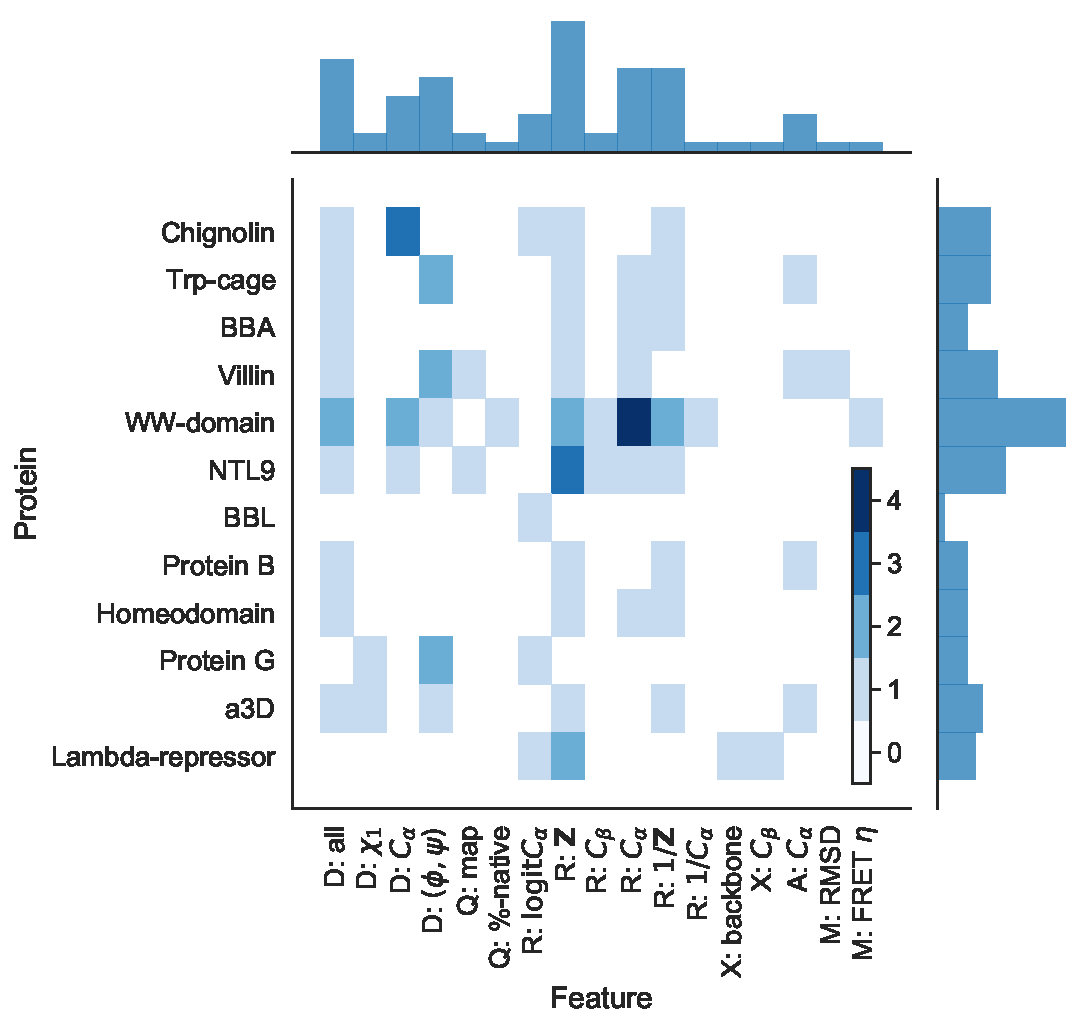
\includegraphics[width=0.9\textwidth]{figures/background_features.pdf}
%     \caption{Proteins studied (vertical) and features selected (horizontal) in every paper using the desres data with MSMs.  D = dihedrals, Q = contacts, R = inter-residue distances, X = positions, A = proper angles.  Z = heavy atoms.  so the most popular feature is the inter residue  distances measured on heavy atoms. The most common protein/feature combination is WW-domain with inter residue distance measured on alpha carbons (4 papers). }
%     \label{fig:my_label}
% \end{figure}


% \section{Introduction}

% Markov state models (MSM) continue to be a popular tool for determining collective variables, kinetic and thermodynamics of complex dynamical systems. Starting with a set of molecular dynamic (MD) simulations, a series of processing steps is performed to create trajectories of discrete states. Using these, the probabilities of state-to-state transitions, separated by a time $\tau$, are estimated giving a discrete approximation to the system's Markov operator. Finally, its eigenvectors and eigenvalues, which represent the relaxation processes and their timescales, are used to extract all relevant kinetic and thermodynamic information. In particular the $k$ slow relaxation processes, separated from the fast relaxation processes by a significant gap in their implied timescales, define the metastable states and contribute most to observables of interest. The accuracy of the model is then strongly influenced by how well the discrete basis states are able to capture these slow eigenvectors. The processing steps, or hyperparameters, which determine the discrete states must therefore be chosen with care. 

% Over the past decade  a firm theoretical foundation for estimating and tuning MSM hyperparameters has been established. The variational approach to conformational dynamics (VAC) established choosing  basis states able to capture the slow Markov eigenvectors as an variational optimisation problem. The generalized matrix Rayleigh coefficient (GMRQ) was introduced which allowed the scoring of hyperparameter choices while avoiding over-fitting with cross-validation. The variational approach to Markov processes (VAMP) generalized VAC to encompass nonreversible dynamics and extended the number of scoring functions. 

% These theoretical developments helped establish the following MSM construction pipeline:  first, an appropriate feature ($\chi$) of the system is chosen which  captures its slow dynamics. For example, the flexible backbone torsion angles of a peptide for protein folding. After `featurizing' the trajectories, a small number ($m$) of linear combinations of these features which approximates the slow dynamics are estimated using  time-independent component analysis (TICA) with a given lag time ($\tau_{\mathrm{TICA}}$). Clustering using e.g., k-means, is used to create $n$ discrete Markov states and estimate the Markov state model. The VAMP score of the MSM can then be used to judge the values of $\chi, m, \tau_{\mathrm{TICA}}$ and $n$ (collectively $\mathbf{x}$). The process of choosing $\mathbf{x}$, fitting an MSM and evaluating using VAMP scores can be repeated until satisfactory convergence of VAMP scores, a process known as hyperparameter tuning. 

% Husic et. al. were among the first to explicitly apply hyperparameter tuning to the problem of MSMs by randomly sampling hyperparameters and selecting the model with the highest cross-validated GMRQ. Scherer et. al. developed a multifidelity tuning approach, by first scoring the featurized trajectories using an approximate VAMP score without estimating a full MSM. This allows selection of a protein feature before going on to tune other hyperparameters. While these approaches were important steps towards a truly reproducible and transparent method for estimating MSMs, several practical questions remain unanswered. First, at what point is convergence in the VAMP scores reached? Second, how can one efficiently reach the optimum values of VAMP scores and hyperparameters? 

% The machine learning community have been active in answering these questions where large machine learning models can take hour or days to train, precluding the ability to exhaustively search the space of potential hyperparameter combinations.  Bayesian optimisation has proven itself a powerful technique for optimising functions, $f(\cdot)$, which are expensive to evaluate with no gradient information (so called ``black-box`` functions). The core of the BO method for hyperparameter optimisation is to model the response of a model (e.g., the VAMP scores of an MSM) to its hyperparameters (e.g., $\mathbf{x}$) with a statistical regression model: $\hat{f}(\mathbf{x})$. At each stage, $i$,  of the optimisation processes, a value of the hyperparameter vector $\mathbf{x}^{i}$ is chosen which is expected to optimise $\hat{f}_{i-1}(\mathbf{x})$. $\mathbf{x}^{i}$ is then evaluated by the model i.e., $f(\theta^{i})$ and this result used to reestimate the response function $\hat{f}_{i}(\mathbf{x})$.  this process continues until the optimum of $\hat{f}$ reaches some convergence criteria. As noted in [firstorder paper] however, Bayesian optimisation is not always guaranteed to be more efficient than randomly sampling hyperparameters, as in [husic].  Thus the first aim of this paper is to both demonstrate how to use BO to optimise MSMs and when it is necessary.  

% However, the VAMP scores themselves are not the objects of interest when creating an MSM.  Typically one is interested in determining metastable states, reactive pathways and their implied timescales.  Nor are VAMP scores the only measure of model quality, importantly they do not address the fundamental assumption for accurate dimensionality reduction - namely a strong separation or gap in the eigenvalue spectrum or implied timescales [tiwary refs, sgoop etc.].  Indeed, the number of dominant eigenvectors which are evaluated in the VAMP score is itself  hyperparameter of the modelling process - but one for which there is no optimisation principal to guide its selection.  It is possible then to optimise a VAMP score but miss important slow processes by selecting too few eigenvectors; or to choose hyperparameters which optimise many fast processes at the expense of the dominant eigenvectors, by choosing too many eigenvectors. 
% In addition, it is not clear how MSM hyperparameters affect the eigenvalue separation and thus the validity of the model.  

% The second aim of this paper is to determine how optimising VAMP scores, in particular in the case where the VAMP score itself is mis-specified, affects the fundamental assumption of a spectral gap. To do this, we extend the response surface modelling used for Bayesian optimisation to describe the sensitivity of the spectral gap to hyperparameters and the VAMP score. 


% Question 1: Do different feature correspond to different models? 
% Question 2: Does different VAMP scores correspond to different models? 
% Question 3: For a given feature, do other hyperparameters matter? 
% Question 4: How sensitive are model observables and VAMP scores to hps? 

% Q1 and 2 answered by compare-path-chart.ipynb



% \section{Materials and methods}

% \subsection{Generating MSM response data}

% \begin{table}
%     \caption{Per protein simulation and analysis parameters}
%     \begin{tabularx}{\textwidth}{llXXXX}
%     \toprule
%     Name & PDB & Simulation time (\si{\micro\second}) & Average folding time (\si{\micro\second}) & No. Residues & Time step (\si{\nano\second}) \\
%      Chignolin           & cln025    & \num{106}     & \num{0.6} & 10 & \num{1} \\
%     Trp-cage            & 2JOF      & \num{208}     & \num{14}  & 20 & \num{1} \\
%     BBA                 & 1FME      & \num{325}     & \num{18}  & 28 & \num{1} \\
%     Villin              & 2F4K      & \num{125}     & \num{2.8} & 35  &\num{1} \\
%     WW domain           & 2F21      & \num{1137}    & \num{21}  & 35 & \num{1} \\
%     NTL9                & 2HBA      & \num{2936}    & \num{29}  & 39  &\num{1} \\
%     BBL                 & 2WXC      & \num{429}     & \num{29}  & 47  &\num{1} \\
%     Protein B           & 1PRB      & \num{104}     & \num{3.9} & 47 & \num{1} \\
%     Homeodomain         & 2P6J      & \num{327}     & \num{3.1} & 52 & \num{1} \\
%     Protein G           & 1MIO      & \num{1154}    & \num{65}  & 56  &\num{1} \\
%     a3D                 & 2A3D      & \num{707}     & \num{27}  & 73  &\num{1} \\
%     $\lambda$-repressor & 1LMB      & \num{643}     & \num{49}  & 80  &\num{1} \\
%     \bottomrule
%     \end{tabularx}
%     \label{tab:data_description}
% \end{table}






% \subsection{Response surface modelling}\label{sec:meth_gp_fit}

% Response surfaces were modelled separately for each combination of protein and feature.  The response surface was modelled as a latent Gaussian processes with additive Gaussian noise:
% \begin{equation}
%     \mathbf{y} \sim \mathcal{N}(\bm{\mu}_{i},\mathbf{K} + \sigma_{n}^{2}\mathbf{I}) \
% \end{equation}
% Where $\mathbf{x}_{i}$ is the $i$'th vector of hyperparameters contained in $\mathcal{D}$; $\bm{\mu}_{i}$ is the mean value of the latent GP at  $\mathbf{x}_{i}$;  $K_{ij}$ is the covariance between observation $i$ and $j$; $\sigma_{n}^{2}$ is the variance of the additive noise;  $y_{i}$ is the measured response (e.g., VAMP($k=2$)) of the MSM trained using the hyperparameters defined by $\mathbf{x}_{i}$. 

% The covariance between the observations was modelled with a stationary kernel of the form: 
% \begin{align}\label{eqn:kernel_form}
%     K_{i, j} + \delta_{i, j}\sigma_{n}^{2} = & \\
%     k\left(\left|\mathbf{x}_{i}-\mathbf{x}_{j}\right|; \theta\right) = &
%     \eta^{2}\prod_h k_{M}\left(\left|x^{h}_{i}-x^{h}_{j}\right|; \nu, l_i\right) + \delta_{i, j}\sigma_{n}^{2}
% \end{align}
% where the product $h$ runs over individual elements of $\mathbf{x}$ (i.e., $\chi, m, \ldots$).  The kernel $k_{M}$ on the individual hyperparameters was a Mat\'ern kernel with roughness parameter $\nu = 3/2$: 
% \begin{equation}
%     k_{\text{M3-2}}\left(r; \sfrac{3}{2}\right) = \exp (-\sqrt{3} r)(1+\sqrt{3} r) \label{eqn:kern_m32}
% \end{equation}
% where, 
% \begin{equation}
%     r = \frac{|x_{i}-x_{j}|}{l}.
% \end{equation}

% Weakly informative priors were placed on the kernel hyperparameters, $\eta$, $\sigma$, and $l$. The prior distributions for the variance terms, $\eta$ and $\sigma$, were $\mathrm{half-Cauchy}(\beta=2)$ and the priors for the length-scale parameters, $l_{i}$, were $\mathrm{Gamma}(\alpha=1, \beta=0.05)$. The r\^ole of weakly informative priors is to exclude unrealistic or disallowed values of the parameters without imposing strong prior beliefs on the true values \cite{gelmanBayesianDataAnalysis2014}. The half-Cauchy distribution  was used for $\eta$ and $\sigma_n$  based on its recommended use in other settings \cite{polsonHalfCauchyPriorGlobal2012}. It was only necessary for the scale of this distribution to give significant density in the range $0-10$ as the VAMP scores will lie in the range $[1,10]$ thus limiting the possible values of $\eta$ and $\sigma_{n}$. The prior for $l$ was justified on the basis that, after scaling the predictors to lie in $[0, 1]$, values of $l \gg 1$ imply a flat response, meaning significant density for $l \gg 1$ isn't necessary. 

% The elements of each  observation of hyperparameters $\mathbf{x}$ were optionally warped by applying a log transformation to make the stationary assumption more accurate. After warping the variables, the value of $\mathbf{x}$ were centered and scaled to the interval $[0, 1]$. So for response surfaces with three MSM hyperparameters, eight potential response functions were considered. The model with the lowest mean standardised log loss were selected. 

% The model parameters ($\bm{\mu}$) and kernel hyperparameters $\theta = (\sigma_n, \eta, l_{i})$ are estimated by maximising the marginal likelihood of the model, $p(\mathbf{y}|\mathcal{D})$ [reference for marginal likelihood] or by Bayesian estimation. 




% All GP modelling was performed with the Python package PyMC3 (version 3.5) \cite{salvatierProbabilisticProgrammingPython2016}.

%  \subsection{MSM hyperparameter relevance}
 
% The stationary and fully multiplicative kernel allows us to identify the inverse of the kernel hyperparameters $l_{i}$ (one for each dimension/hyperparameter) with the the relevance:
% \begin{equation}
%     R_{i} = \frac{1}{l_{i}}
% \end{equation}
% The value of $R_{i}$ is learned in the fitting process and determines how sensitive the MSM response is to variation in the MSM-hyperparameter, $x_{i}$. For $R_{i} \simeq 0$ small changes in the $i$'th hyperparameter,  $x_{i}$, make little difference the MSM response, $y$; as $R \gg 1$, small changes in $x_{i}$ make large differences to $y$. 

% A Bayesian approach was used to estimate the GP parameters and hyperparameters (and hence the relevance) using MCMC with No-U-Turn sampler.  4 independent chains with 1000 tuning steps and 1000 sampling steps were used. Convergence was checked using the criteria set out in \cite{vehtariRanknormalizationFoldingLocalization2020}.  

% \subsection{Bayesian optimisation}

% The response surface of an MSM can be optimised using Bayesian optimisation and requires two ingredients: i) a response function which models the response of the MSM to its hyperparameters, and ii) an acquisition function. We used a GP model for the response function. The acquisition function we used is the expected improvement, $\mathbb{E}\left[I\right]$. The improvement, $I$, is defined as \cite{shahriariTakingHumanOut2016}:
% \begin{equation}
%     I(\mathbf{x}, \mu^{*}):=(f(\mathbf{x}) - \mu^{*}) \mathbb{I}_{f(\mathbf{x}) > \mu^{*}}.
% \end{equation}
% Taking the expectation of this for a Gaussian process gives \cite{shahriariTakingHumanOut2016}:
% \begin{align}\label{eqn:msm_ei_def}
%         \alpha_{EI}(\mathbf{x}) := &  \mathbb{E}\left[I(\mathbf{x}, f(\mathbf{x}), \mu^{*})\right] \\
%          =  &(\mu(\mathbf{x}) - \mu^{*})\Phi\left( \frac{ \mu(\mathbf{x}) - \mu^{*} }{\sigma(\mathbf{x})} \right ) + \sigma(\mathbf{x})\phi\left( \frac{ \mu(\mathbf{x}) - \mu^{*} }{\sigma(\mathbf{x}) } \right )
% \end{align}
% Here $\Phi,\ \phi$ are the normal cumulative and probability distribution functions respectively, and $\sigma(\mathbf{x})^{2}$ is the variance of the GP at the point $\mathbf{x}$. It is possible to take the expectation over both the distribution of $f$ and of the GP hyperparameters $\theta$. This has been suggested and shown to be effective \cite{NIPS2012_4522}. However, it was not clear whether the extra accuracy warranted the extra computational costs. 

% The Bayesian optimisation algorithm \cite{shahriariTakingHumanOut2016} starts with a hyperparameter trial data set of size $N_{\mathrm{seed}}$ which we used to estimate an initial response surface $f(\mathbf{x}; \mathcal{D}_{N_{\mathrm{seed}}})$ and calculate the incumbent: 
% \begin{equation}
%     \mu^{*}(\mathbf{x}^{*}) = \max{\left[f(\mathbf{x})\right]},\ \mathbf{x}\in \mathcal{D}_{N_{\mathrm{seed}}}
% \end{equation}
% The incumbent we take to mean the maximum of the response surface \emph{measured at observed hyperparameter values}. This means that information from all hyperparameter trials is incorporated. 

% In step 1 of the algorithm, a candidate hyperparameter $\mathbf{x}_{1}$ is chosen by finding the maximum of the acquisition function using the BGFS algorithm with 100 random restarts.  The response, $y_{1}$, of the MSM to this candidate was calculated, and the trial $(\mathbf{x}_{1}, y_{1})$ added to the trial data set, which becomes  $\mathcal{D}_{N_{\mathrm{seed}}+1}$. This process is repeated for $p$ steps and is summarised in in algorithm \ref{alg:bayes_opt}.

% \begin{algorithm}
% \KwData{Trial data: $\mathcal{D}_{N} = \{(y_{1}, \mathbf{x}_{1}), ...,(y_{N}, \mathbf{x}_{N})\}$}
% \KwData{Search space grid: $\mathbf{X}_{\mathrm{M}} = \{(\chi_1, \tau_1, m_1, n_1), ...,(\chi_{M}, \tau_{M}, m_{M}, n_{M})\}$}
% \KwResult{$\mathbf{x}^{*} = \argmax_{\mathbf{x}}{f(\mathbf{x}; \mathcal{D}_{N+p})}$}
% \BlankLine
% \For{$i\leftarrow N$ \KwTo $N+p$}{
%     estimate GP response $f(\mathbf{x}; \mathcal{D}_{i})$\;
%     calculate incumbent: $\mu^{*} = \argmax{f(\mathbf{x};\mathcal{D}_{i})}\ \mathrm{s.t.}\ (y, \mathbf{x}) \in \mathcal{D}_{i}$\;
%     estimate acquisition function: $\alpha_{\mathrm{EI}}(\mathbf{x}; \mathcal{D}_{i})\ \mathbf{x} \in \mathbf{X}$\;
%     select candidate: $\mathbf{x}_{i+1} = \argmax_{\mathbf{x}}\alpha_{\mathrm{EI}}(\mathbf{x}; \mathcal{D}_{i})\ \mathrm{s.t.}\ (\mathbf{x} \in \mathbf{X})\ \&\ (\mathbf{x} \notin \mathcal{D}_{i})$\;
%     query objective function to obtain: $y_{i+1}$\;
%     augment data: $\mathcal{D}_{i+1} \leftarrow \{\mathcal{D}_{i}, (y_{i+1}, \mathbf{x}_{i+1})\}$
% }
% \caption{Bayesian Optimisation.\label{alg:bayes_opt}}
% \end{algorithm}


% % \printbibliography



% \section{Results and discussion}



% \subsection{Markov lag time}

% The Markov lag time is usually chosen by inspection of an implied timescale plot to find the smallest lag time such that the dominant ($t_{2}$) timescale is constant. The VAMP scores, which will be used to rank the hyperparameter choices, also depend on the lag time. However, implied timescales, and therefore the lag time, are dependent on the definition of the microstates and hence the hyperparameters. We are therefor in a situation where in order to choose hyperparameters we need to specify a lag time, but an appropriate lag time can only be found once suitable set of hyperparameter is found. To mitigate this circular problem the lag time was chosen by inspection of $t_{2}$ as a function of the lag time $\tau$ for \emph{all} hyperparameter choices (trials). The lag time was chosen as the smallest value such the lag time gradient was less than 


% \subsection{How do hyperparameters affect VAMP scores? }

% Context - do we need to worry about searching hyperparameters for the best combination? 

% % \begin{figure}
% %     \centering
% %     \includegraphics[width=0.8\textwidth]{figures/wild-mouse-photography-4.jpg}
% %     \caption{Top  VAMP scores for each protein/feature combination.}
% %     \label{fig:1}
% % \end{figure}


% % \begin{figure}
% %     \centering
% %     \includegraphics[width=0.8\textwidth]{figures/wild-mouse-photography-4.jpg}
% %     \caption{Relevance of hyperparameters to properly specified VAMP scores.}
% %     \label{fig:2}
% % \end{figure}


% Comments: 
% \begin{enumerate}
%     \item Expect to see differences in fig 1. i.e., we know some features are better for protein folding that others. 
%     \item Expect to see most hyperparameters do not affect VAMP scores. 
%     \item 'properly specified' means the VAMP score is only measured on the truly dominant timescales. 
% \end{enumerate}
 

% \subsection{How do hyperparameters affect model validity?}

% Context - unknown whether hyperparameters affect other aspects of MSMs

% \begin{figure}
%     \centering
%     \includegraphics[width=0.8\textwidth]{figures/wild-mouse-photography-4.jpg}
%     \caption{relevance of hyperparameters to spectral gap (i.e., repeat of Fig2 but with gap instead of VAMP) }
%     \label{fig:4}
% \end{figure}


% Comments: 
% \begin{enumerate}
%     \item I suspect (from experience) that mis-specifying VAMP scores will affect this. e.g., if there are really 2 dominant processes, but you optimise the top 1 processes, then you may not get a good separation of timescales.  
%     \item I'm not sure the extent to which we care about separation of timescales in the same way as I don't know how much we should care about high VAMP scores.  
%     \item Possibly drop this - but seems to tie in nicely with recent discussions on model validity. See: https://aip.scitation.org/doi/10.1063/5.0030931
% \end{enumerate}


% \section{Conclusions}

% \clearpage
% \section{Figures}

% Move to SI. 

% \clearpage
% \subsection{Choosing the Markov lag-time}

% \begin{figure}[h]
%     \centering
%     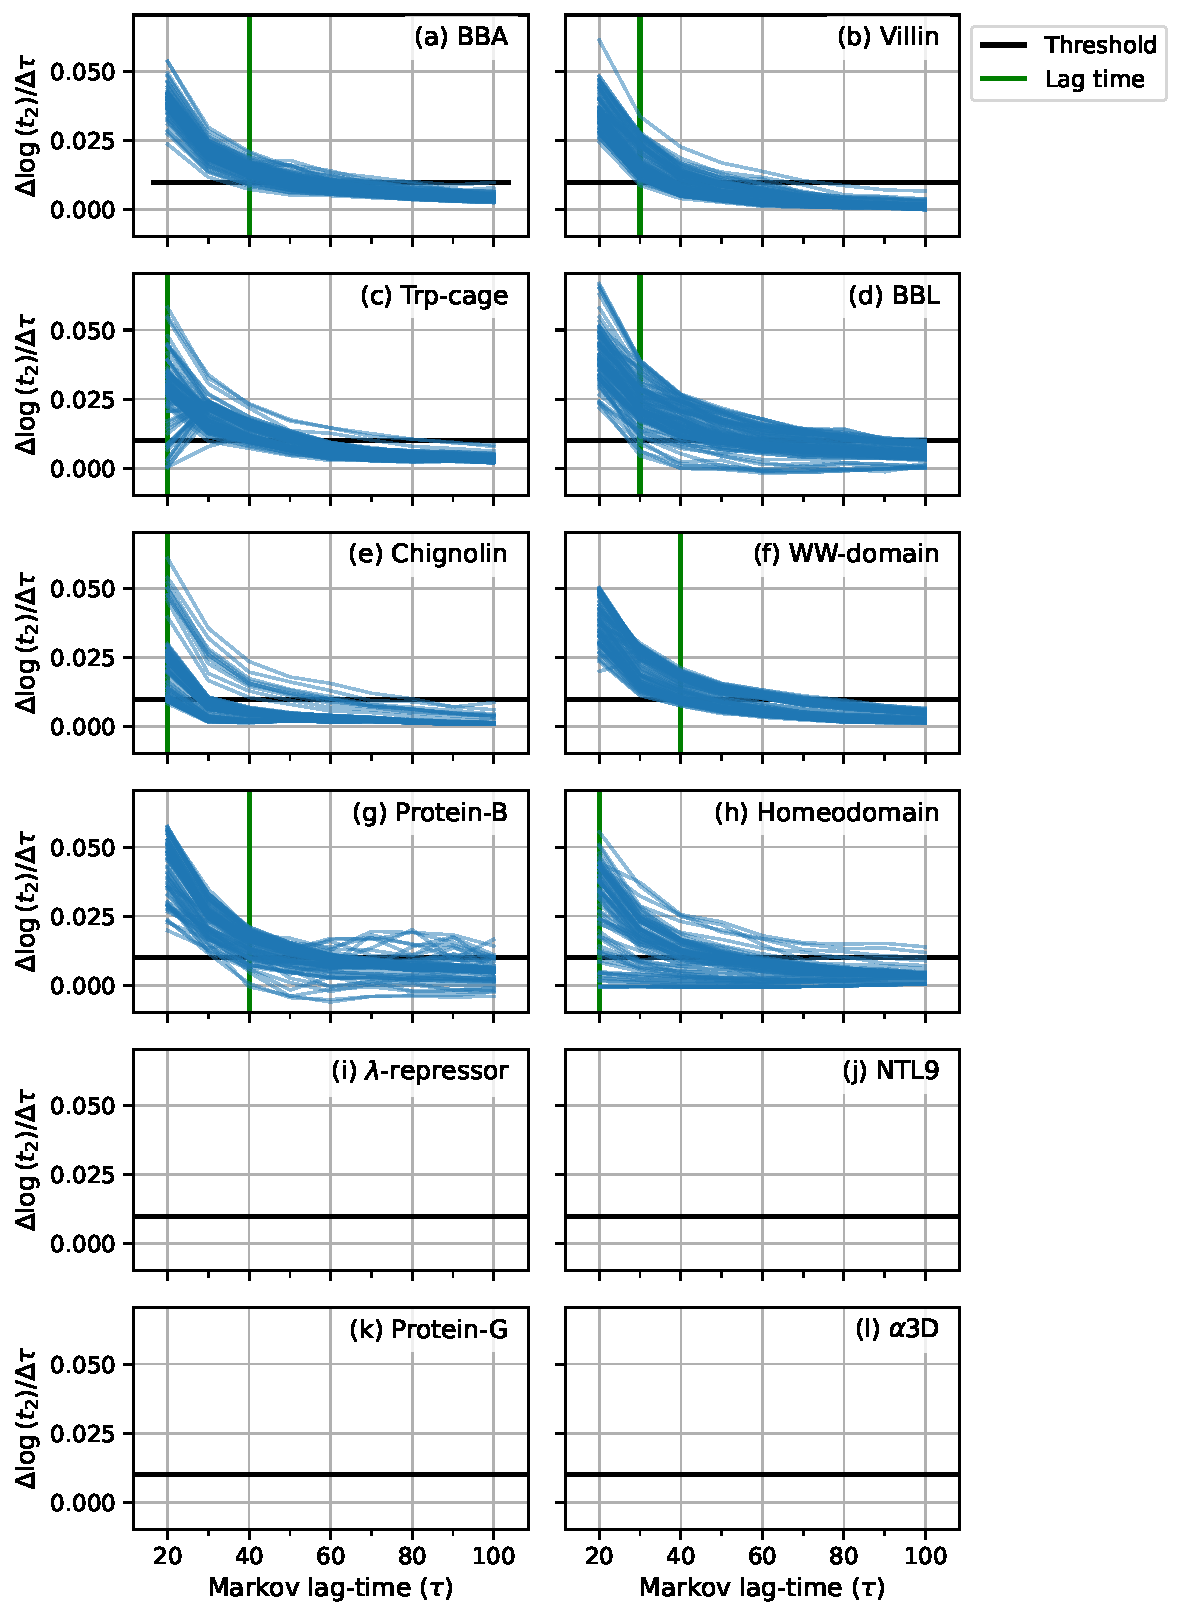
\includegraphics[height=0.65\textheight]{figures/t_2_gradient_sharey_True_log_True_denom_delta_x.pdf}
%     \caption{\textsc{Implied timescale gradient for all hyperparameter trials.} Each panel shows $\Delta t_{2}/\Delta \tau$: gradient of the dominant timescale ($t_{2}$) with respect to the Markov lag-time. The gradient was calculated for each bootstrap sample and then the median was taken. The horizontal black line is the threshold for determining the lag time. The vertical blue line is the chosen lag-time.}
%     \label{fig:t2_gradient}
% \end{figure}

% \clearpage
% \subsection{Choosing the number of dominant processes}



% \clearpage
% \subsection{BBA}

% \begin{table}[h]
%     \centering
%     \begin{tabular}{lllll}
%     \toprule
%     Model &               1 &               2 &               3 &               4 \\
%     \midrule
%     Rank                             &               1 &               3 &              35 &             100 \\
%     VAMP-2 score                     &           3.882 &           3.873 &           3.723 &           2.505 \\
%     VAMP-2 \SI{95}{\percent} C.I.    &  [3.840, 3.905] &  [3.834, 3.899] &  [3.631, 3.807] &  [2.442, 2.562] \\
%     Num. eigenvectors                &               4 &               4 &               4 &               4 \\
%     Lag (ns)                         &              40 &              40 &              40 &              40 \\
%     Feature                          &       Distances &       Distances &       Dihedrals &       Distances \\
%     Contact scheme                   &       C$\alpha$ &       C$\alpha$ &               - &   Closest-Heavy \\
%     Transform                        &        Logistic &          Linear &               - &        Logistic \\
%     Logistic center (\si{\angstrom}) &            0.61 &            0.80 &               - &            1.33 \\
%     Logistic steepness               &           24.72 &            8.26 &               - &           17.37 \\
%     TICA lag (ns)                    &              63 &              84 &              45 &              87 \\
%     TICA dimension                   &               6 &              10 &               9 &               1 \\
%     Num. clusters                    &             349 &             260 &             291 &              96 \\
%     \bottomrule
%     \end{tabular}
%     \caption{\textsc{Summary of comparator models for BBA.} Models 1, 2, and 3 are the best scoring model for each feature/transform combination, model 4 is the worst performing model of all features.  The performance of the model is determined by its rank in terms of its median VAMP-2 score.  The chosen Markov lag time is determined from figure \ref{fig:t2_gradient} and number of dominant eigenvectors from figure \ref{fig:count_num_proc}, these are the same for each model by construction. The hyperparameters which specify the mapping of trajectories to microstates are also listed.}
%     \label{tab:1fme_mod_defs}
% \end{table}


% \begin{figure}[h]
%     \centering
%     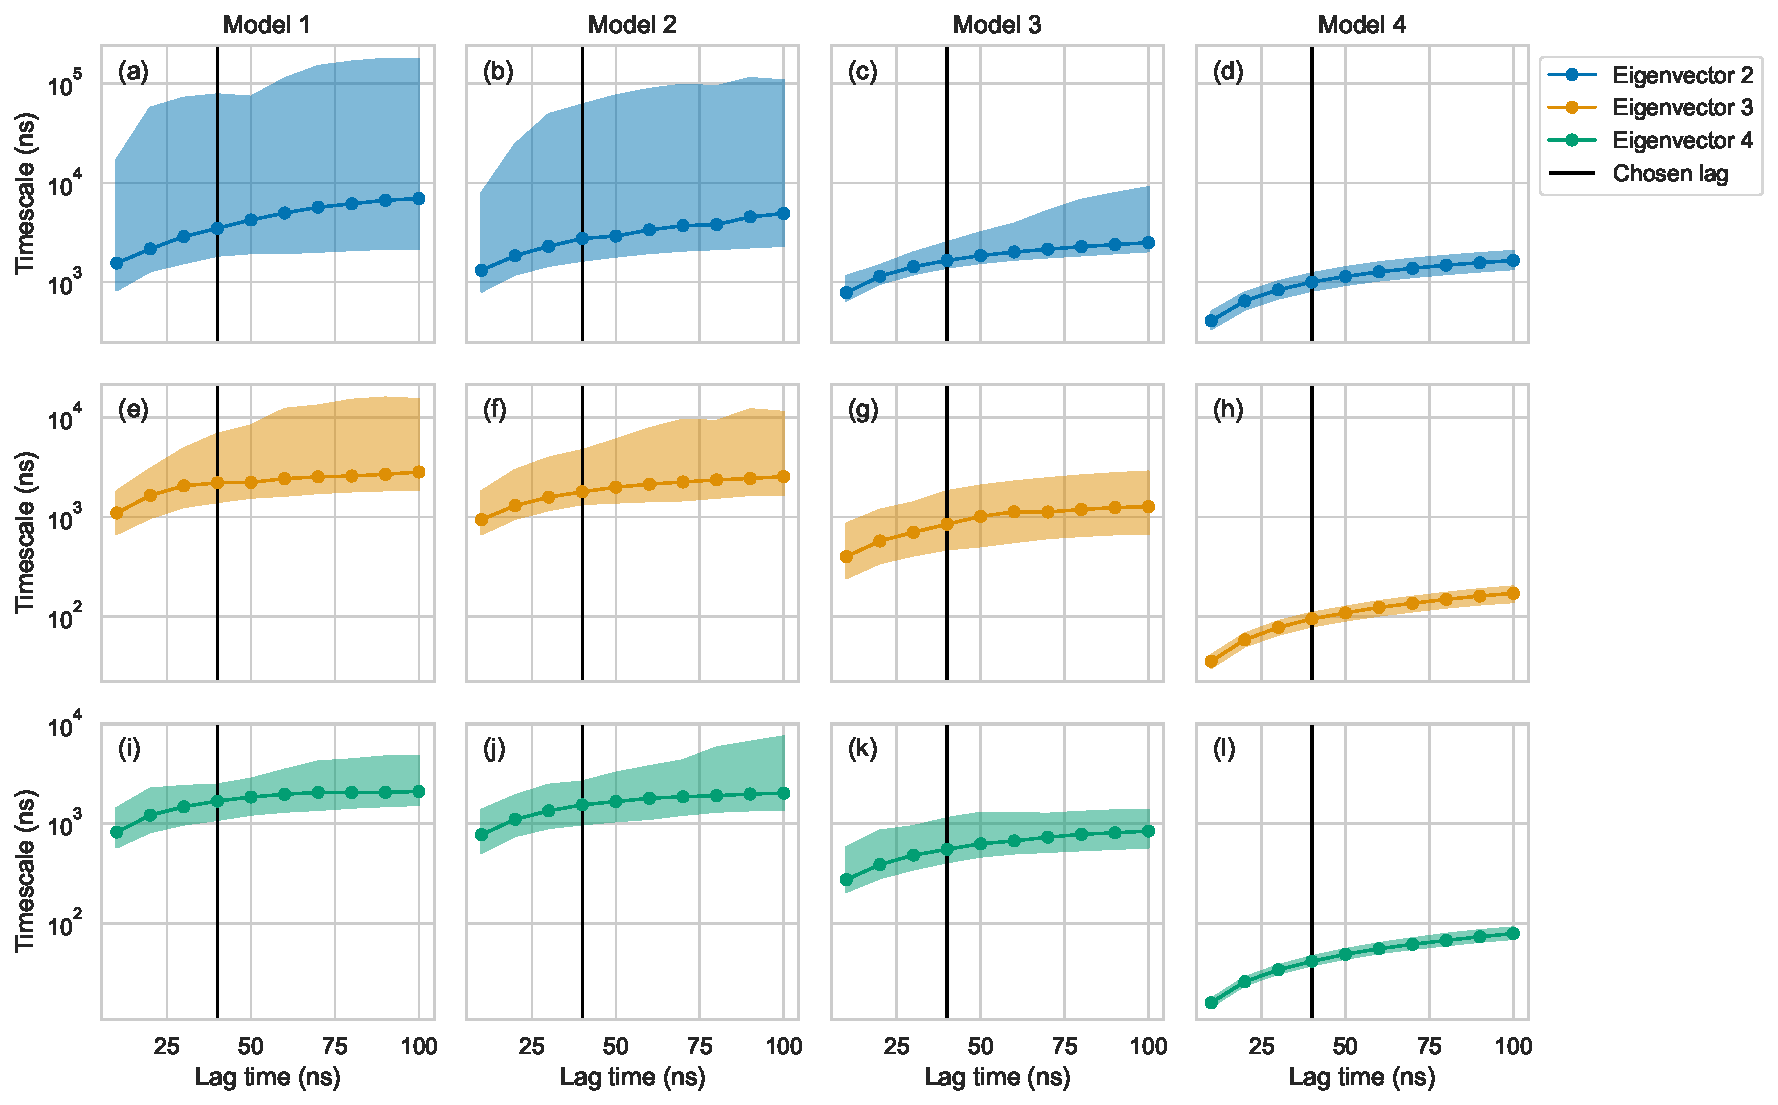
\includegraphics[width=1\textwidth]{figures/model_comparision_its/1fme.pdf}
%     \caption{\textsc{Implied timescales of BBA for comparator models.} Panels (a) - (d) correspond to models 1 - 4 which are specified in table \ref{tab:1fme_mod_defs}. Panels (a), (e) and (i) show the implied timescales for the 2nd, 3rd and 4th eigenvectors for model 1, which are the dominant eigenvectors identified in figure \ref{fig:count_num_proc}.  Panels (b), (f) and (j) show the implied timescales for model 2 and so on.}
%     \label{fig:1fme_its}
% \end{figure}


% \begin{figure}[h]
%     \centering
%     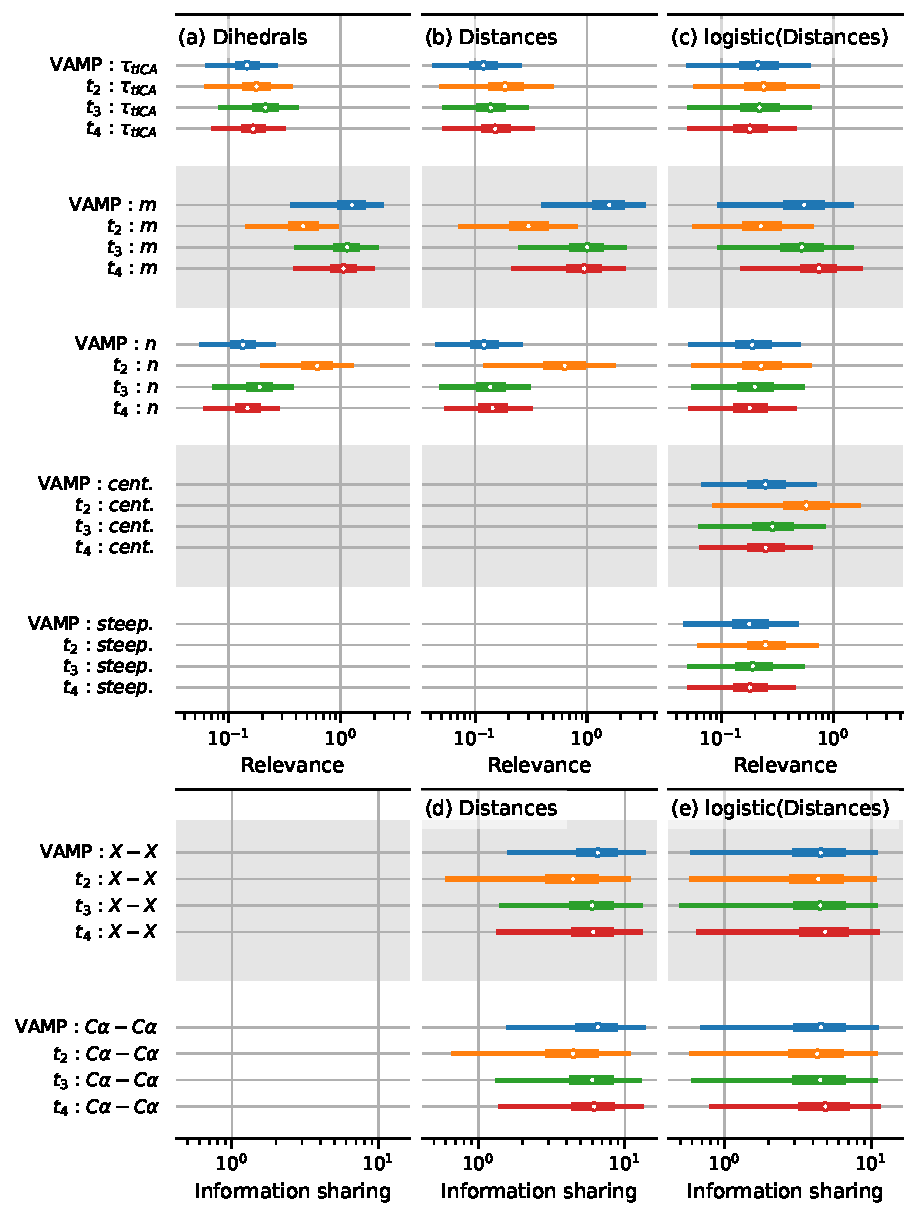
\includegraphics[height=0.8\textheight]{figures/sensitivities/1fme_sensitivity.pdf}
%     \caption{\textsc{BBA hyperparameter relevance and information sharing}. Shown are the  median (white dot), \SI{50}{\percent} and \SI{95}{\percent} credible intervals (thick and thin lines respectively).  Panels (a)-(c) show the hyperparameter relevance for of each hyperparameter in determining the log of the VAMP-2 score (`VAMP' in blue) and the log of the dominant timescales ($t_{2}, t_{3}, ...$ in orange, green etc.). $\tau_{\mathrm{tICA}}$ is the TICA lag-time; $m$ is the TICA dimension, $n$ is the number of cluster centers; $cent.$ and $steep.$ are the center and steepness parameters of the logistic transform. Panels (d)-(e) show the information sharing parameters for whether the contact distances use the `closest-heavy' ($X-X$) or the `alpha-carbon' ($C_{\alpha}-C_{\alpha}$) scheme.}
%     \label{fig:1fme_sense}
% \end{figure}


% \clearpage
% \subsection{Villin}

% \begin{table}[h]
%     \centering
%     \begin{tabular}{lllll}
%     \toprule
%     Model &               1 &               2 &               3 &               4 \\
%     \midrule
%     Rank                             &               1 &               4 &              26 &              99 \\
%     VAMP-2 score                     &           2.773 &           2.758 &           2.741 &           1.496 \\
%     VAMP-2 \SI{95}{\percent} C.I.    &  [2.682, 2.806] &  [2.649, 2.796] &  [2.627, 2.783] &  [1.422, 1.648] \\
%     Num. eigenvectors                &               3 &               3 &               3 &               3 \\
%     Lag (ns)                         &              30 &              30 &              30 &              30 \\
%     Feature                          &       Distances &       Dihedrals &       Distances &       Distances \\
%     Contact scheme                   &       C$\alpha$ &               - &   Closest-Heavy &       C$\alpha$ \\
%     Transform                        &          Linear &               - &        Logistic &        Logistic \\
%     Logistic center (\si{\angstrom}) &            1.49 &               - &            0.59 &            0.38 \\
%     Logistic steepness               &           17.87 &               - &            2.40 &           38.49 \\
%     TICA lag (ns)                    &              16 &               6 &              21 &              79 \\
%     TICA dimension                   &               8 &               6 &               5 &               9 \\
%     Num. clusters                    &             291 &             458 &             296 &             300 \\
%     \bottomrule
%     \end{tabular}
%     \caption{\textsc{Summary of comparator models for villin.} Models 1, 2, and 3 are the best scoring model for each feature/transform combination, model 4 is the worst performing model of all features.  The performance of the model is determined by its rank in terms of its median VAMP-2 score.  The chosen Markov lag time is determined from figure \ref{fig:t2_gradient} and number of dominant eigenvectors from figure \ref{fig:count_num_proc}, these are the same for each model by construction. The hyperparameters which specify the mapping of trajectories to microstates are also listed.}
%     \label{tab:2f4k_mod_defs}
% \end{table}


% \begin{figure}[h]
%     \centering
%     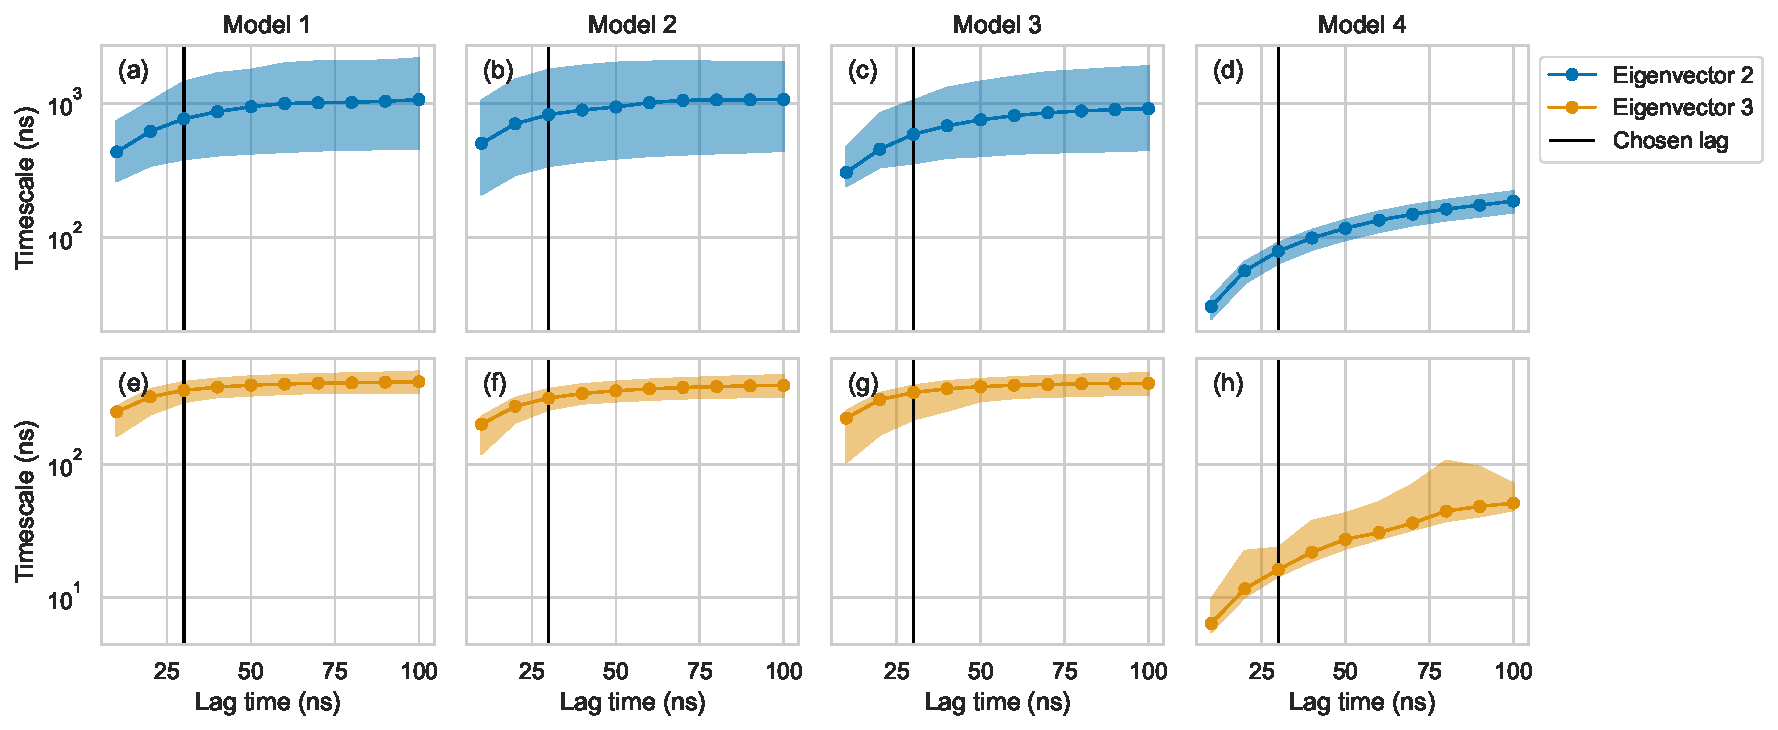
\includegraphics[width=1\textwidth]{figures/model_comparision_its/2f4k.pdf}
%     \caption{\textsc{Implied timescales of villin for comparator models.} Panels (a) - (d) correspond to models 1 - 4 which are specified in table \ref{tab:1fme_mod_defs}. Panels (a), (e) and (i) show the implied timescales for the 2nd, 3rd and 4th eigenvectors for model 1, which are the dominant eigenvectors identified in figure \ref{fig:count_num_proc}.  Panels (b), (f) and (j) show the implied timescales for model 2 and so on.}
%     \label{fig:2f4k_its}
% \end{figure}


% \begin{figure}[h]
%     \centering
%     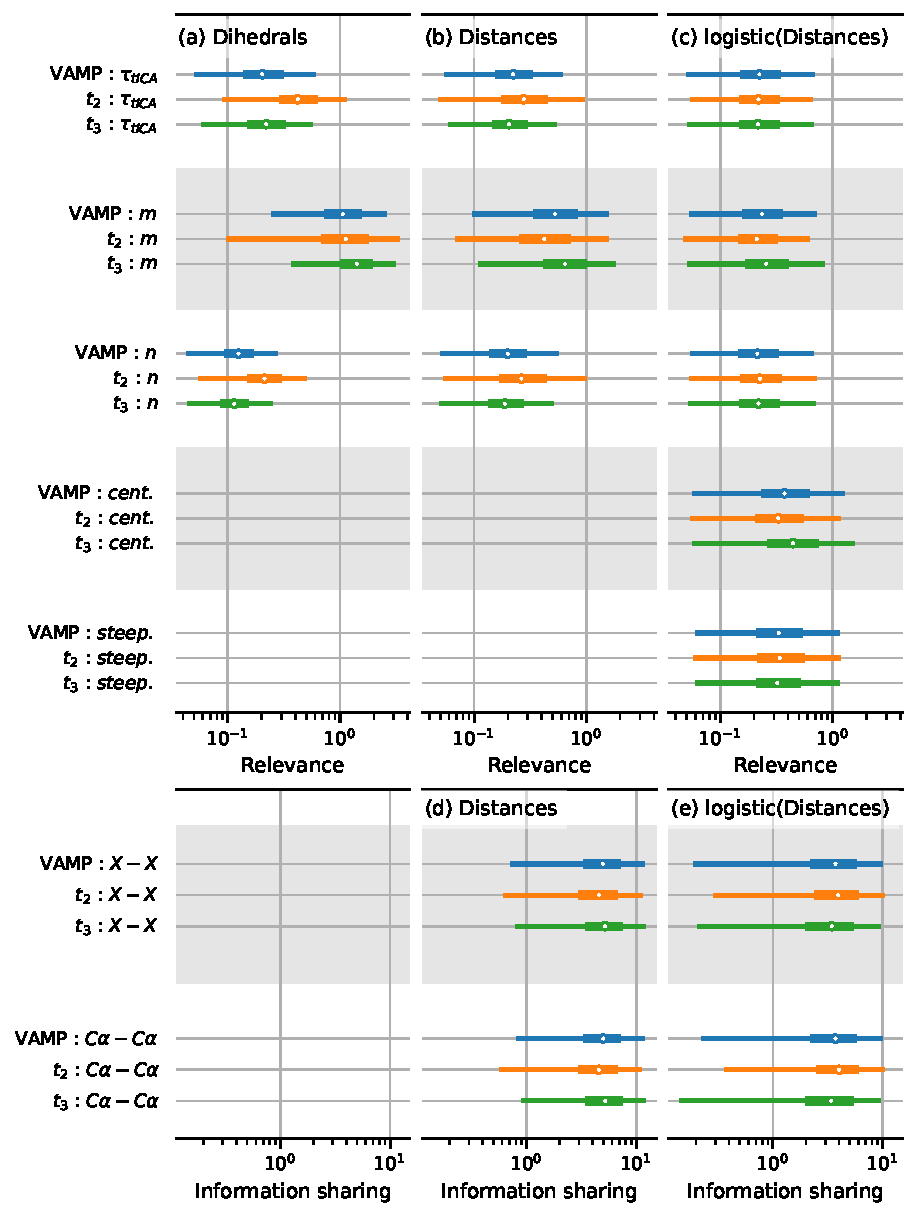
\includegraphics[height=0.8\textheight]{figures/sensitivities/2f4k_sensitivity.pdf}
%     \caption{\textsc{Villin hyperparameter relevance and information sharing}. Shown are the  median (white dot), \SI{50}{\percent} and \SI{95}{\percent} credible intervals (thick and thin lines respectively).  Panels (a)-(c) show the hyperparameter relevance for of each hyperparameter in determining the log of the VAMP-2 score (`VAMP' in blue) and the log of the dominant timescales ($t_{2}, t_{3}, ...$ in orange, green etc.). $\tau_{\mathrm{tICA}}$ is the TICA lag-time; $m$ is the TICA dimension, $n$ is the number of cluster centers; $cent.$ and $steep.$ are the center and steepness parameters of the logistic transform. Panels (d)-(e) show the information sharing parameters for whether the contact distances use the `closest-heavy' ($X-X$) or the `alpha-carbon' ($C_{\alpha}-C_{\alpha}$) scheme.  }
%     \label{fig:2f4k_sense}
% \end{figure}

% \clearpage
% \subsection{Trp-cage}

% \begin{table}[h]
%     \centering
%     \begin{tabular}{lllll}
%     \toprule
%     Model &               1 &               2 &               3 &               4 \\
%     \midrule
%     Rank                             &               1 &              46 &              56 &             100 \\
%     VAMP-2 score                     &           2.931 &           2.884 &           2.870 &           2.017 \\
%     VAMP-2 \SI{95}{\percent} C.I.    &  [2.725, 2.950] &  [2.828, 2.926] &  [2.804, 2.912] &  [1.993, 2.056] \\
%     Num. eigenvectors                &               3 &               3 &               3 &               3 \\
%     Lag (ns)                         &              20 &              20 &              20 &              20 \\
%     Feature                          &       Dihedrals &       Distances &       Distances &       Distances \\
%     Contact scheme                   &               - &       C$\alpha$ &       C$\alpha$ &   Closest-Heavy \\
%     Transform                        &               - &          Linear &        Logistic &        Logistic \\
%     Logistic center (\si{\angstrom}) &               - &            1.21 &            0.49 &            1.33 \\
%     Logistic steepness               &               - &           42.49 &            1.45 &           17.37 \\
%     TICA lag (ns)                    &               1 &              66 &              83 &              87 \\
%     TICA dimension                   &              10 &               6 &               9 &               1 \\
%     Num. clusters                    &             298 &             421 &              70 &              96 \\
%     \bottomrule
%     \end{tabular}
%     \caption{\textsc{Summary of comparator models for Trp-cage.} Models 1, 2, and 3 are the best scoring model for each feature/transform combination, model 4 is the worst performing model of all features.  The performance of the model is determined by its rank in terms of its median VAMP-2 score.  The chosen Markov lag time is determined from figure \ref{fig:t2_gradient} and number of dominant eigenvectors from figure \ref{fig:count_num_proc}, these are the same for each model by construction. The hyperparameters which specify the mapping of trajectories to microstates are also listed.}
%     \label{tab:2jof_mod_defs}
% \end{table}


% \begin{figure}[h]
%     \centering
%     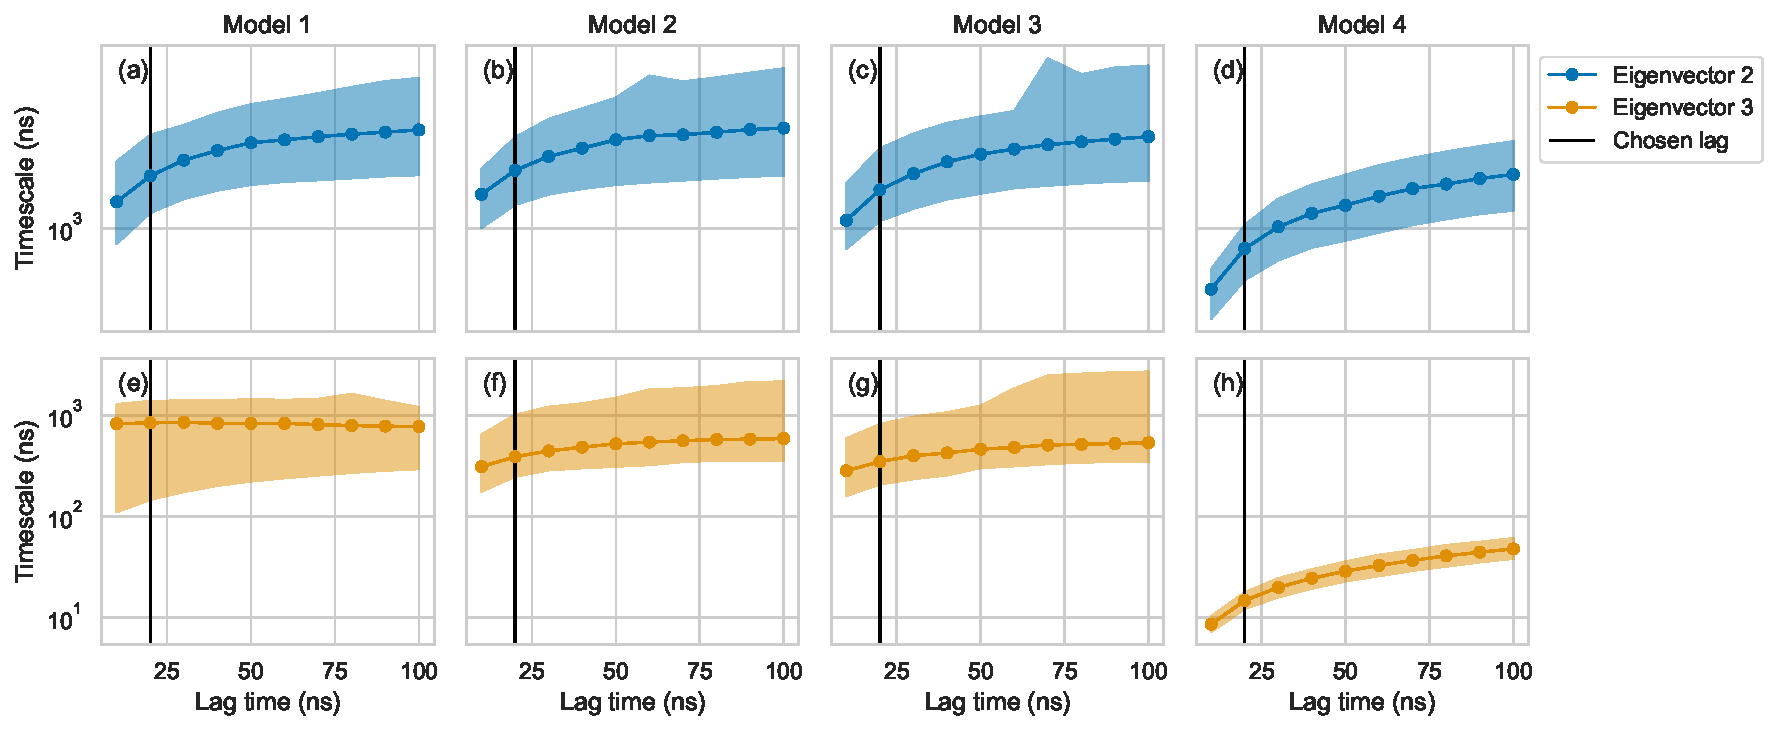
\includegraphics[width=1\textwidth]{figures/model_comparision_its/2jof.pdf}
%     \caption{\textsc{Implied timescales of Trp-cage for comparator models.} Panels (a) - (d) correspond to models 1 - 4 which are specified in table \ref{tab:1fme_mod_defs}. Panels (a), (e) and (i) show the implied timescales for the 2nd, 3rd and 4th eigenvectors for model 1, which are the dominant eigenvectors identified in figure \ref{fig:count_num_proc}.  Panels (b), (f) and (j) show the implied timescales for model 2 and so on.}
%     \label{fig:2jof_its}
% \end{figure}

% \begin{figure}[h]
%     \centering
%     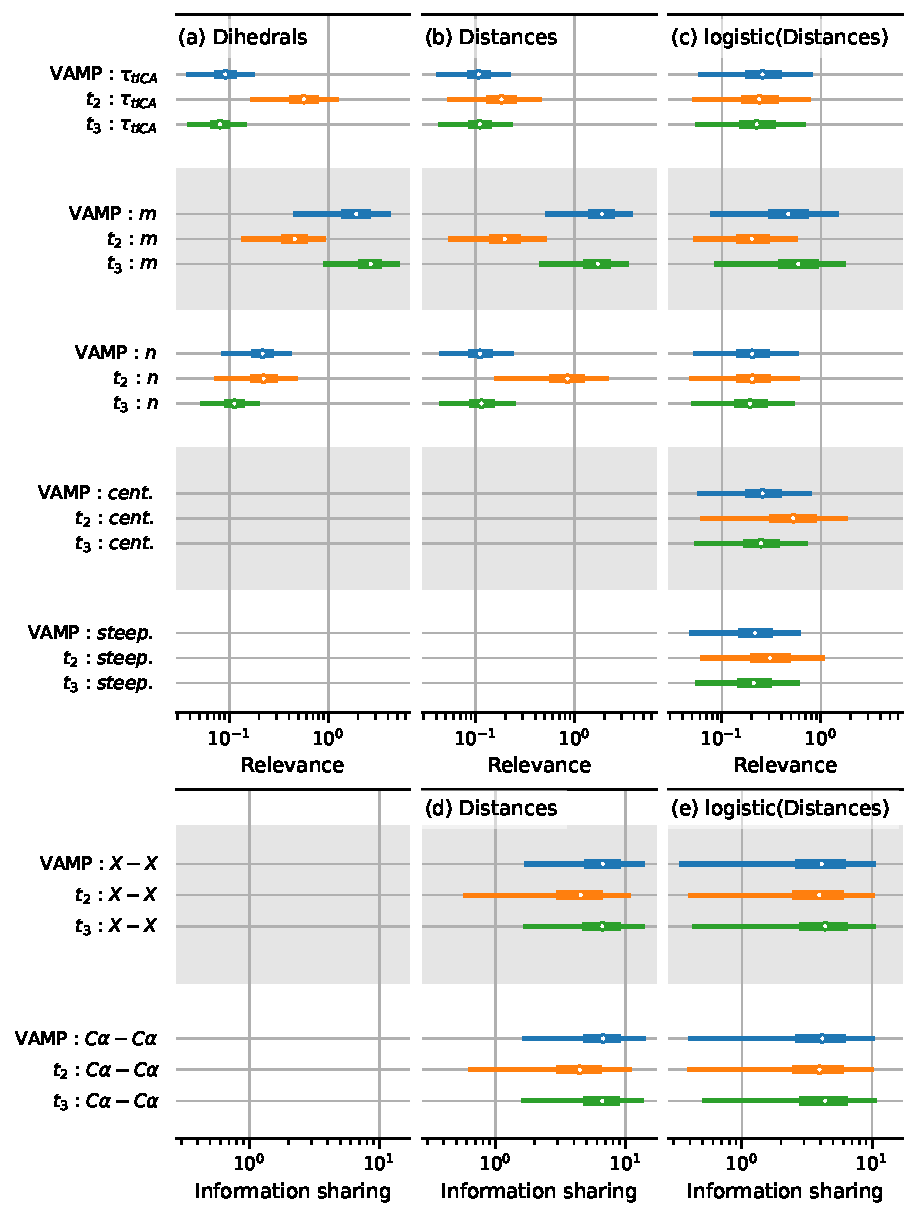
\includegraphics[height=0.8\textheight]{figures/sensitivities/2jof_sensitivity.pdf}
%     \caption{\textsc{Trp-cage hyperparameter relevance and information sharing}. Shown are the  median (white dot), \SI{50}{\percent} and \SI{95}{\percent} credible intervals (thick and thin lines respectively).  Panels (a)-(c) show the hyperparameter relevance for of each hyperparameter in determining the log of the VAMP-2 score (`VAMP' in blue) and the log of the dominant timescales ($t_{2}, t_{3}, ...$ in orange, green etc.). $\tau_{\mathrm{tICA}}$ is the TICA lag-time; $m$ is the TICA dimension, $n$ is the number of cluster centers; $cent.$ and $steep.$ are the center and steepness parameters of the logistic transform. Panels (d)-(e) show the information sharing parameters for whether the contact distances use the `closest-heavy' ($X-X$) or the `alpha-carbon' ($C_{\alpha}-C_{\alpha}$) scheme.  }
%     \label{fig:2jof_sense}
% \end{figure}

% \clearpage
% \subsection{BBL}

% \begin{table}[h]
%     \centering
%     \begin{tabular}{lllll}
%     \toprule
%     Model &               1 &               2 &               3 &               4 \\
%     \midrule
%     Rank                             &               1 &               2 &              13 &              97 \\
%     VAMP-2 score                     &           2.991 &           2.989 &           2.988 &           1.009 \\
%     VAMP-2 \SI{95}{\percent} C.I.    &  [2.975, 2.998] &  [2.969, 2.997] &  [2.973, 2.995] &  [1.004, 1.067] \\
%     Num. eigenvectors                &               3 &               3 &               3 &               3 \\
%     Lag (ns)                         &              30 &              30 &              30 &              30 \\
%     Feature                          &       Dihedrals &       Distances &       Distances &       Dihedrals \\
%     Contact scheme                   &               - &       C$\alpha$ &       C$\alpha$ &               - \\
%     Transform                        &               - &          Linear &        Logistic &               - \\
%     Logistic center (\si{\angstrom}) &               - &            0.83 &            1.06 &               - \\
%     Logistic steepness               &               - &           21.27 &           11.70 &               - \\
%     TICA lag (ns)                    &              33 &              44 &              71 &              95 \\
%     TICA dimension                   &              10 &               9 &              10 &               1 \\
%     Num. clusters                    &             311 &             316 &             447 &             111 \\
%     \bottomrule
%     \end{tabular}
%     \caption{\textsc{Summary of comparator models for BBL.} Models 1, 2, and 3 are the best scoring model for each feature/transform combination, model 4 is the worst performing model of all features.  The performance of the model is determined by its rank in terms of its median VAMP-2 score.  The chosen Markov lag time is determined from figure \ref{fig:t2_gradient} and number of dominant eigenvectors from figure \ref{fig:count_num_proc}, these are the same for each model by construction. The hyperparameters which specify the mapping of trajectories to microstates are also listed.}
%     \label{tab:2wav_mod_defs}
% \end{table}

% \begin{figure}[h]
%     \centering
%     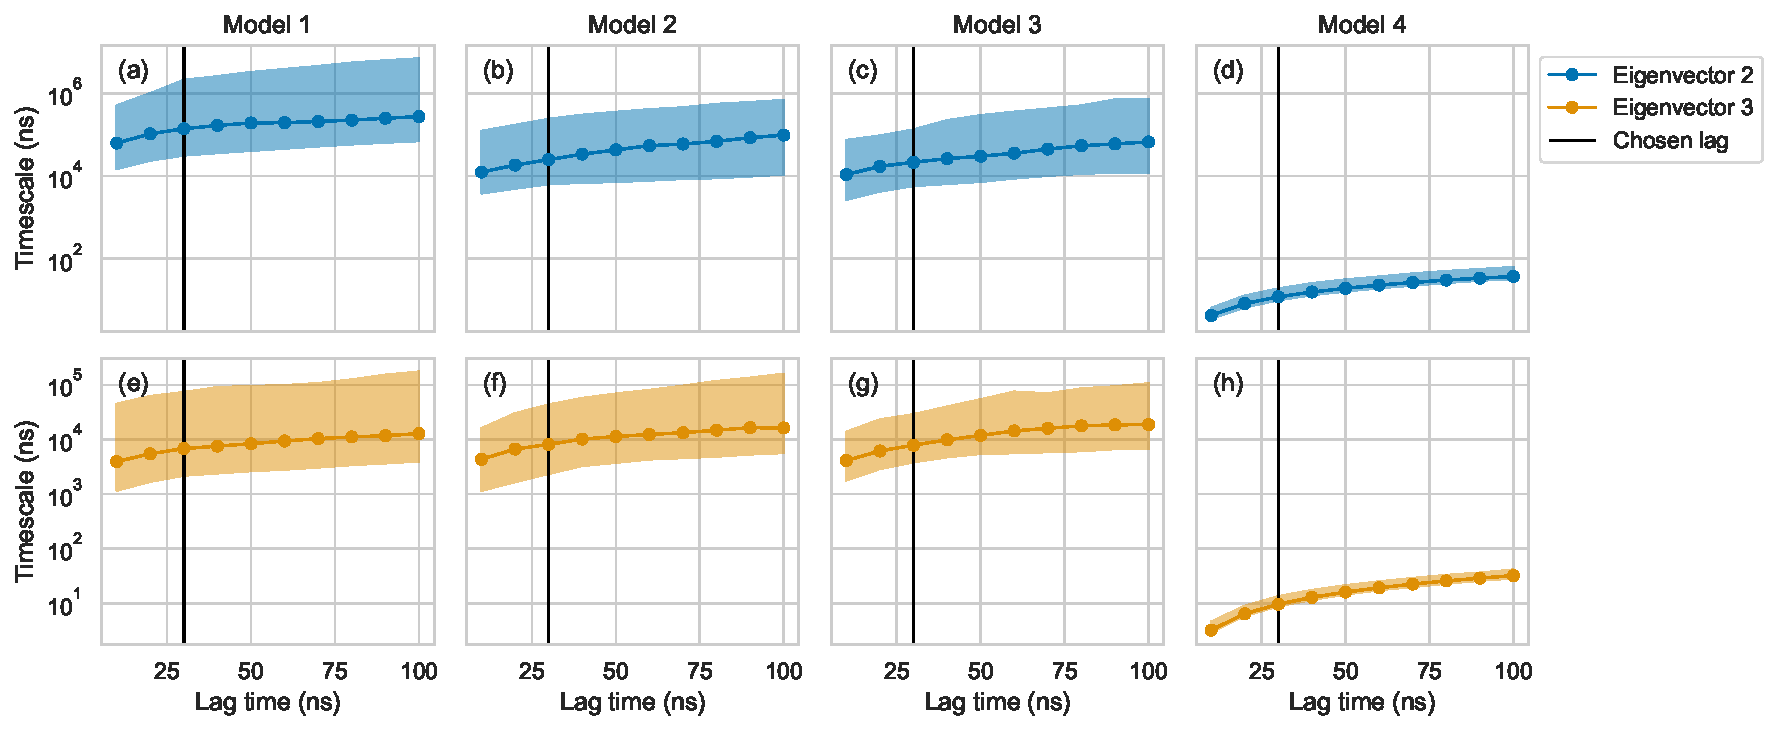
\includegraphics[width=1\textwidth]{figures/model_comparision_its/2wav.pdf}
%     \caption{\textsc{Implied timescales of BBL for comparator models.} Panels (a) - (d) correspond to models 1 - 4 which are specified in table \ref{tab:1fme_mod_defs}. Panels (a), (e) and (i) show the implied timescales for the 2nd, 3rd and 4th eigenvectors for model 1, which are the dominant eigenvectors identified in figure \ref{fig:count_num_proc}.  Panels (b), (f) and (j) show the implied timescales for model 2 and so on.}
%     \label{fig:2wav_its}
% \end{figure}

% \begin{figure}[h]
%     \centering
%     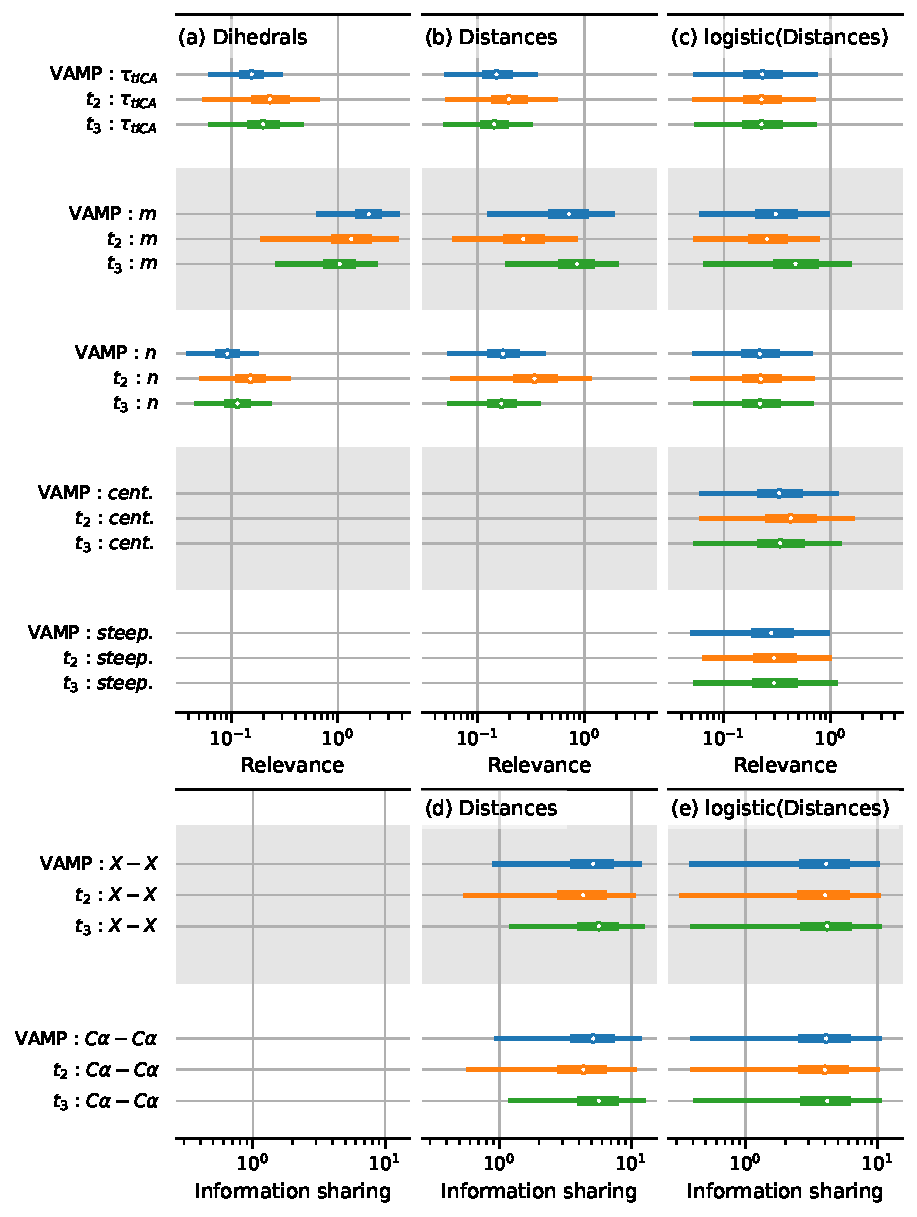
\includegraphics[height=0.8\textheight]{figures/sensitivities/2wav_sensitivity.pdf}
%     \caption{\textsc{BBL hyperparameter relevance and information sharing}. Shown are the  median (white dot), \SI{50}{\percent} and \SI{95}{\percent} credible intervals (thick and thin lines respectively).  Panels (a)-(c) show the hyperparameter relevance for of each hyperparameter in determining the log of the VAMP-2 score (`VAMP' in blue) and the log of the dominant timescales ($t_{2}, t_{3}, ...$ in orange, green etc.). $\tau_{\mathrm{tICA}}$ is the TICA lag-time; $m$ is the TICA dimension, $n$ is the number of cluster centers; $cent.$ and $steep.$ are the center and steepness parameters of the logistic transform. Panels (d)-(e) show the information sharing parameters for whether the contact distances use the `closest-heavy' ($X-X$) or the `alpha-carbon' ($C_{\alpha}-C_{\alpha}$) scheme.  }
%     \label{fig:2wav_sense}
% \end{figure}

% \clearpage
% \subsection{Chignolin}

% \begin{table}[h]
%     \centering
%     \begin{tabular}{lllll}
%     \toprule
%     Model &               1 &               2 &               3 &               4 \\
%     \midrule
%     Rank                             &               1 &              17 &              33 &              99 \\
%     VAMP-2 score                     &           1.898 &           1.895 &           1.890 &           1.300 \\
%     VAMP-2 \SI{95}{\percent} C.I.    &  [1.871, 1.911] &  [1.871, 1.909] &  [1.864, 1.906] &  [1.272, 1.324] \\
%     Num. eigenvectors                &               2 &               2 &               2 &               2 \\
%     Lag (ns)                         &              20 &              20 &              20 &              20 \\
%     Feature                          &       Distances &       Distances &       Dihedrals &       Distances \\
%     Contact scheme                   &   Closest-Heavy &   Closest-Heavy &               - &   Closest-Heavy \\
%     Transform                        &          Linear &        Logistic &               - &        Logistic \\
%     Logistic center (\si{\angstrom}) &            0.41 &            0.59 &               - &            1.49 \\
%     Logistic steepness               &            6.75 &            2.40 &               - &           39.00 \\
%     TICA lag (ns)                    &              13 &              21 &               1 &              77 \\
%     TICA dimension                   &               2 &               5 &              10 &               3 \\
%     Num. clusters                    &             413 &             296 &             298 &              85 \\
%     \bottomrule
%     \end{tabular}
%     \caption{\textsc{Summary of comparator models for chignolin.} Models 1, 2, and 3 are the best scoring model for each feature/transform combination, model 4 is the worst performing model of all features.  The performance of the model is determined by its rank in terms of its median VAMP-2 score.  The chosen Markov lag time is determined from figure \ref{fig:t2_gradient} and number of dominant eigenvectors from figure \ref{fig:count_num_proc}, these are the same for each model by construction. The hyperparameters which specify the mapping of trajectories to microstates are also listed.}
%     \label{tab:cln025_mod_defs}
% \end{table}


% \begin{figure}[h]
%     \centering
%     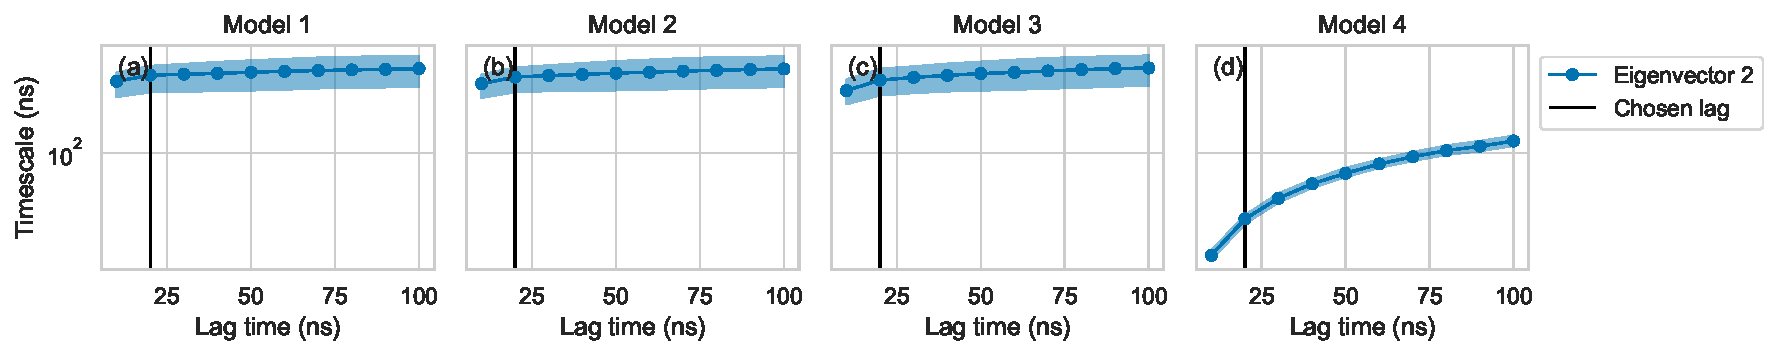
\includegraphics[width=1\textwidth]{figures/model_comparision_its/cln025.pdf}
%     \caption{\textsc{Implied timescales of chignolin for comparator models.} Panels (a) - (d) correspond to models 1 - 4 which are specified in table \ref{tab:1fme_mod_defs}. They show the implied timescales for the 2nd eigenvector for model 1 - 4, which are the dominant eigenvectors identified in figure \ref{fig:count_num_proc}.}
%     \label{fig:cln025_its}
% \end{figure}


% \begin{figure}[h]
%     \centering
%     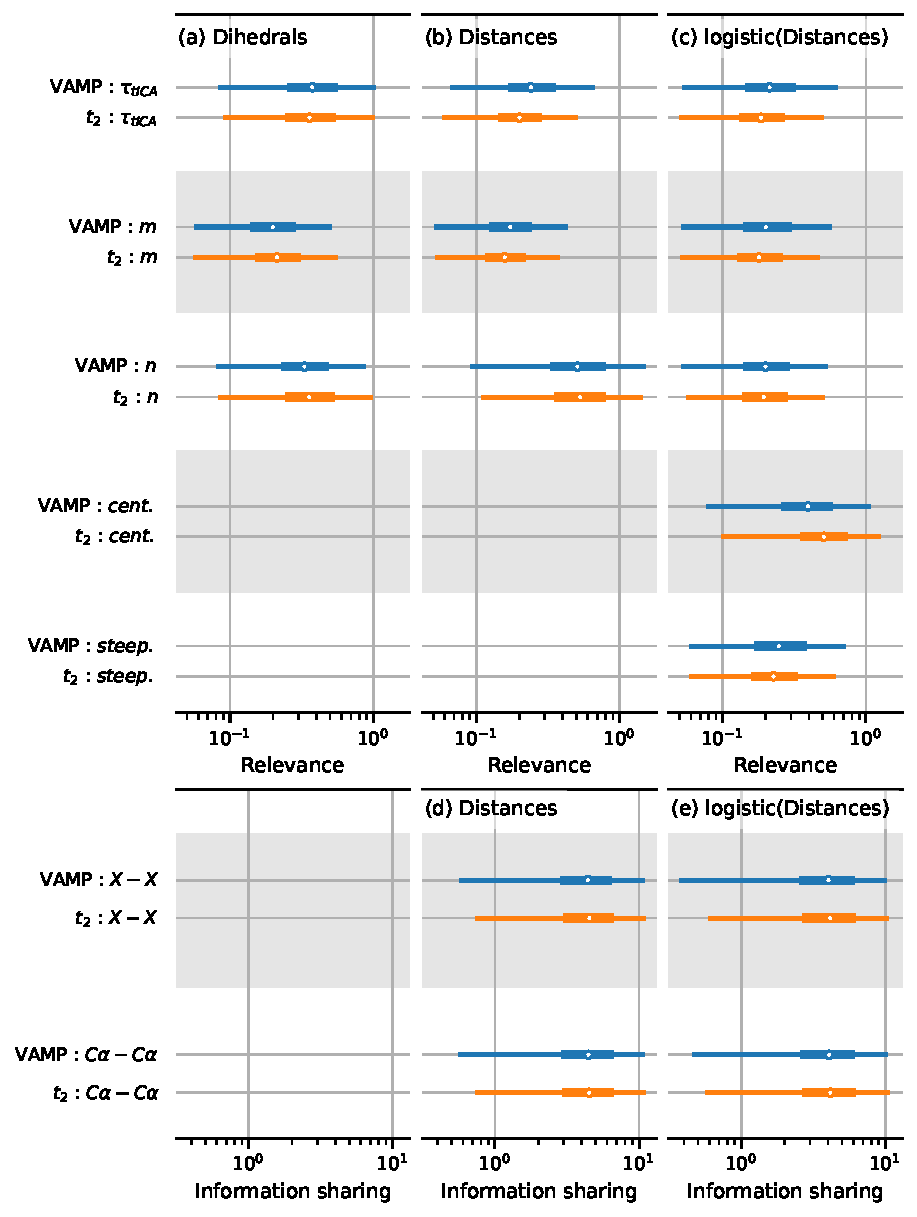
\includegraphics[height=0.8\textheight]{figures/sensitivities/cln025_sensitivity.pdf}
%     \caption{\textsc{Chignolin hyperparameter relevance and information sharing}. Shown are the  median (white dot), \SI{50}{\percent} and \SI{95}{\percent} credible intervals (thick and thin lines respectively).  Panels (a)-(c) show the hyperparameter relevance for of each hyperparameter in determining the log of the VAMP-2 score (`VAMP' in blue) and the log of the dominant timescales ($t_{2}, t_{3}, ...$ in orange, green etc.). $\tau_{\mathrm{tICA}}$ is the TICA lag-time; $m$ is the TICA dimension, $n$ is the number of cluster centers; $cent.$ and $steep.$ are the center and steepness parameters of the logistic transform. Panels (d)-(e) show the information sharing parameters for whether the contact distances use the `closest-heavy' ($X-X$) or the `alpha-carbon' ($C_{\alpha}-C_{\alpha}$) scheme.  }
%     \label{fig:cln025_sense}
% \end{figure}

% \clearpage
% \subsection{WW-domain}

% \begin{table}[h]
%     \centering
%     \begin{tabular}{lllll}
%     \toprule
%     Model &               1 &               2 &               3 &               4 \\
%     \midrule
%     Rank                             &               1 &              42 &              43 &              99 \\
%     VAMP-2 score                     &           3.887 &           3.748 &           3.735 &           2.449 \\
%     VAMP-2 \SI{95}{\percent} C.I.    &  [3.876, 3.897] &  [3.545, 3.814] &  [3.528, 3.861] &  [2.357, 2.860] \\
%     Num. eigenvectors                &               4 &               4 &               4 &               4 \\
%     Lag (ns)                         &              40 &              40 &              40 &              40 \\
%     Feature                          &       Dihedrals &       Distances &       Distances &       Dihedrals \\
%     Contact scheme                   &               - &       C$\alpha$ &       C$\alpha$ &               - \\
%     Transform                        &               - &        Logistic &          Linear &               - \\
%     Logistic center (\si{\angstrom}) &               - &            1.06 &            0.80 &               - \\
%     Logistic steepness               &               - &           11.70 &            8.26 &               - \\
%     TICA lag (ns)                    &              33 &              71 &              84 &              95 \\
%     TICA dimension                   &               2 &              10 &              10 &               1 \\
%     Num. clusters                    &             322 &             447 &             260 &             111 \\
%     \bottomrule
%     \end{tabular}
%     \caption{\textsc{Summary of comparator models for WW-domain.} Models 1, 2, and 3 are the best scoring model for each feature/transform combination, model 4 is the worst performing model of all features.  The performance of the model is determined by its rank in terms of its median VAMP-2 score.  The chosen Markov lag time is determined from figure \ref{fig:t2_gradient} and number of dominant eigenvectors from figure \ref{fig:count_num_proc}, these are the same for each model by construction. The hyperparameters which specify the mapping of trajectories to microstates are also listed.}
%     \label{tab:gtt_mod_defs}
% \end{table}

% \begin{figure}[h]
%     \centering
%     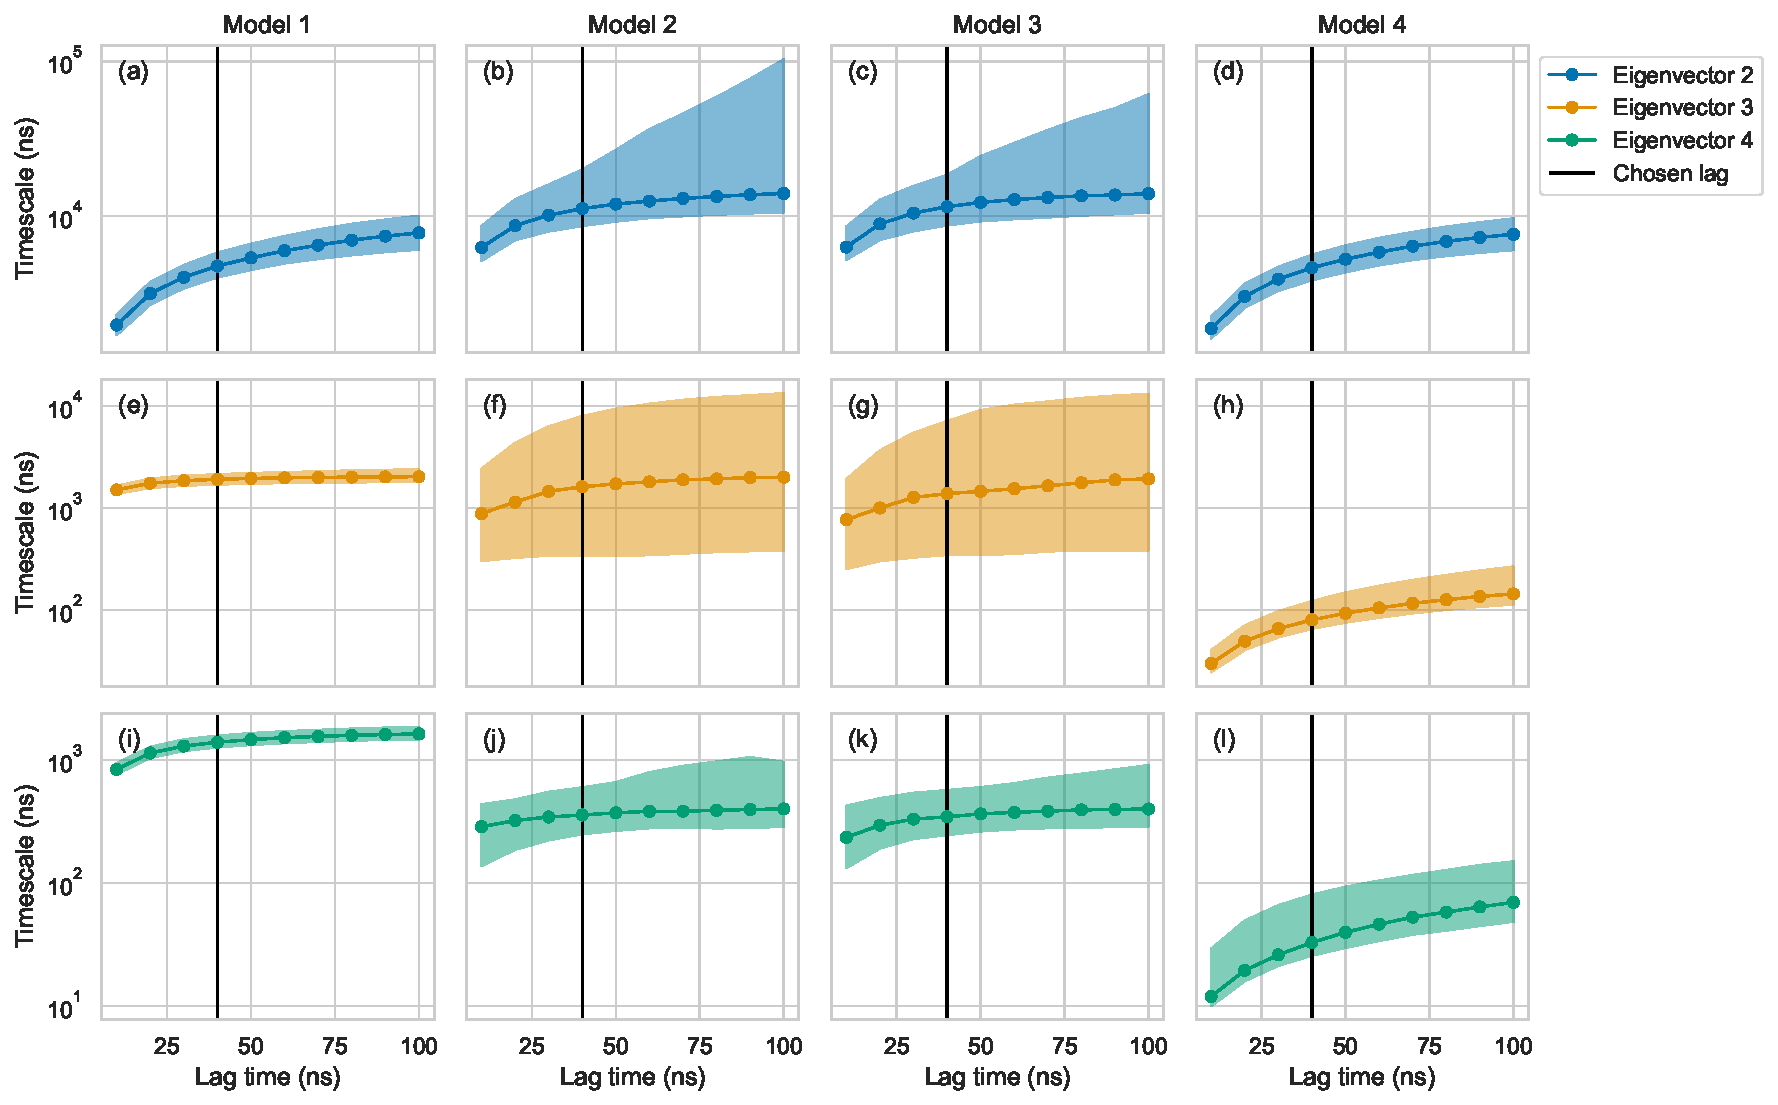
\includegraphics[width=1\textwidth]{figures/model_comparision_its/gtt.pdf}
%     \caption{\textsc{Implied timescales of WW-domain for comparator models.} Panels (a) - (d) correspond to models 1 - 4 which are specified in table \ref{tab:1fme_mod_defs}. Panels (a), (e) and (i) show the implied timescales for the 2nd, 3rd and 4th eigenvectors for model 1, which are the dominant eigenvectors identified in figure \ref{fig:count_num_proc}.  Panels (b), (f) and (j) show the implied timescales for model 2 and so on.}
%     \label{fig:gtt_its}
% \end{figure}


% \begin{figure}[h]
%     \centering
%     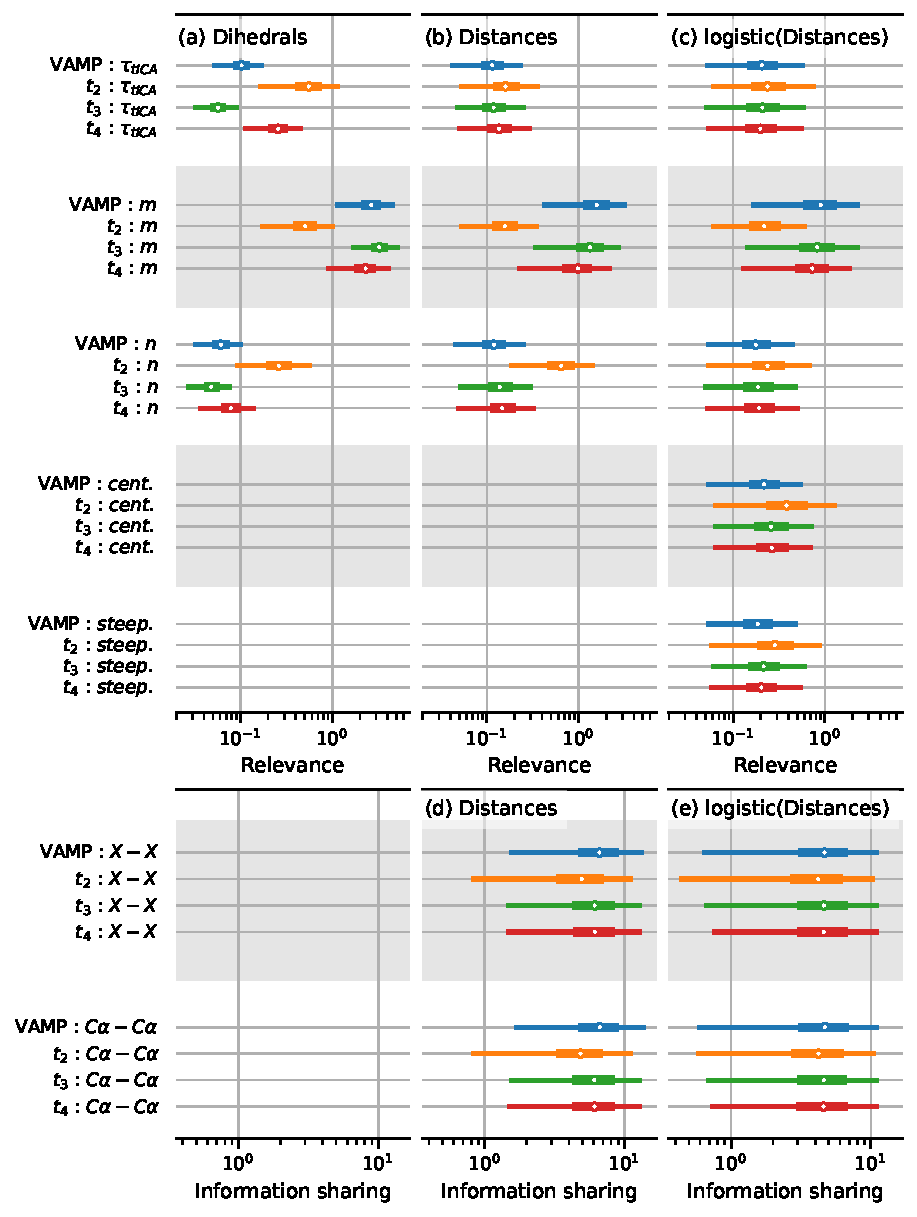
\includegraphics[height=0.8\textheight]{figures/sensitivities/gtt_sensitivity.pdf}
%     \caption{\textsc{WW-domain hyperparameter relevance and information sharing}. Shown are the  median (white dot), \SI{50}{\percent} and \SI{95}{\percent} credible intervals (thick and thin lines respectively).  Panels (a)-(c) show the hyperparameter relevance for of each hyperparameter in determining the log of the VAMP-2 score (`VAMP' in blue) and the log of the dominant timescales ($t_{2}, t_{3}, ...$ in orange, green etc.). $\tau_{\mathrm{tICA}}$ is the TICA lag-time; $m$ is the TICA dimension, $n$ is the number of cluster centers; $cent.$ and $steep.$ are the center and steepness parameters of the logistic transform. Panels (d)-(e) show the information sharing parameters for whether the contact distances use the `closest-heavy' ($X-X$) or the `alpha-carbon' ($C_{\alpha}-C_{\alpha}$) scheme.  }
%     \label{fig:gtt_sense}
% \end{figure}


% \clearpage
% \subsection{Protein-B}
% \begin{table}[h]
%     \centering
%     \begin{tabular}{lllll}
%     \toprule
%     Model &               1 &               2 &               3 &               4 \\
%     \midrule
%     Rank                             &               1 &              12 &              34 &              87 \\
%     VAMP-2 score                     &           2.827 &           2.802 &           2.476 &           1.806 \\
%     VAMP-2 \SI{95}{\percent} C.I.    &  [2.637, 2.910] &  [2.585, 2.890] &  [2.177, 2.639] &  [1.216, 2.286] \\
%     Num. eigenvectors                &               3 &               3 &               3 &               3 \\
%     Lag (ns)                         &              40 &              40 &              40 &              40 \\
%     Feature                          &       Distances &       Distances &       Dihedrals &       Distances \\
%     Contact scheme                   &       C$\alpha$ &       C$\alpha$ &               - &       C$\alpha$ \\
%     Transform                        &          Linear &        Logistic &               - &        Logistic \\
%     Logistic center (\si{\angstrom}) &            1.21 &            0.84 &               - &            0.38 \\
%     Logistic steepness               &           42.49 &           42.84 &               - &           38.49 \\
%     TICA lag (ns)                    &              66 &              76 &              33 &              79 \\
%     TICA dimension                   &               6 &               4 &              10 &               9 \\
%     Num. clusters                    &             421 &             291 &             311 &             300 \\
%     \bottomrule
%     \end{tabular}
%     \caption{\textsc{Summary of comparator models for protein-B.} Models 1, 2, and 3 are the best scoring model for each feature/transform combination, model 4 is the worst performing model of all features.  The performance of the model is determined by its rank in terms of its median VAMP-2 score.  The chosen Markov lag time is determined from figure \ref{fig:t2_gradient} and number of dominant eigenvectors from figure \ref{fig:count_num_proc}, these are the same for each model by construction. The hyperparameters which specify the mapping of trajectories to microstates are also listed.}
%     \label{tab:prb_mod_defs}
% \end{table}

% \begin{figure}[h]
%     \centering
%     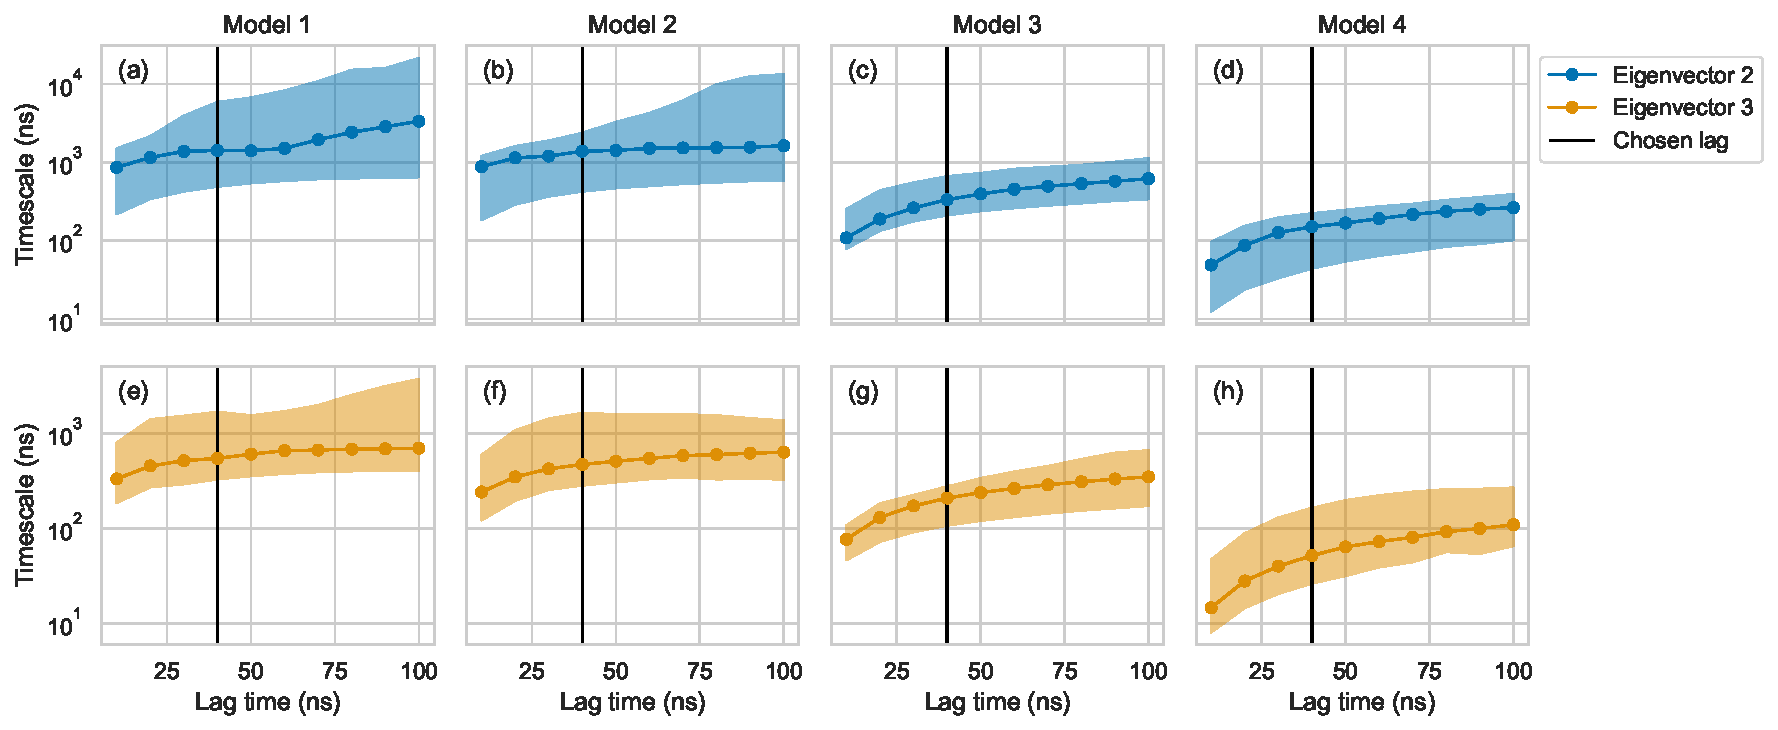
\includegraphics[width=1\textwidth]{figures/model_comparision_its/prb.pdf}
%     \caption{\textsc{Implied timescales of protein-B for comparator models.} Panels (a) - (d) correspond to models 1 - 4 which are specified in table \ref{tab:1fme_mod_defs}. Panels (a), (e) and (i) show the implied timescales for the 2nd, 3rd and 4th eigenvectors for model 1, which are the dominant eigenvectors identified in figure \ref{fig:count_num_proc}.  Panels (b), (f) and (j) show the implied timescales for model 2 and so on.}
%     \label{fig:prb_its}
% \end{figure}

% \begin{figure}[h]
%     \centering
%     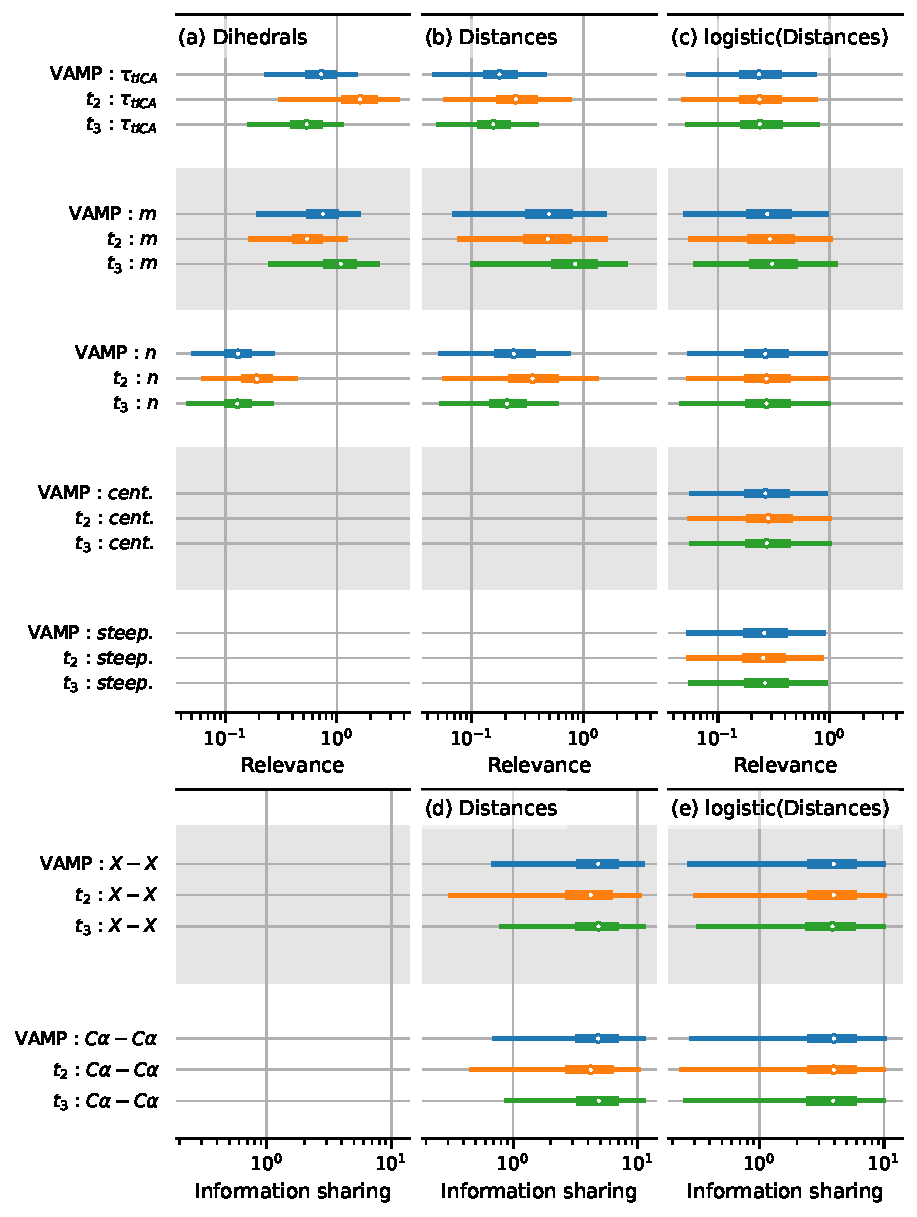
\includegraphics[height=0.8\textheight]{figures/sensitivities/prb_sensitivity.pdf}
%     \caption{\textsc{Protein-B hyperparameter relevance and information sharing}. Shown are the  median (white dot), \SI{50}{\percent} and \SI{95}{\percent} credible intervals (thick and thin lines respectively).  Panels (a)-(c) show the hyperparameter relevance for of each hyperparameter in determining the log of the VAMP-2 score (`VAMP' in blue) and the log of the dominant timescales ($t_{2}, t_{3}, ...$ in orange, green etc.). $\tau_{\mathrm{tICA}}$ is the TICA lag-time; $m$ is the TICA dimension, $n$ is the number of cluster centers; $cent.$ and $steep.$ are the center and steepness parameters of the logistic transform. Panels (d)-(e) show the information sharing parameters for whether the contact distances use the `closest-heavy' ($X-X$) or the `alpha-carbon' ($C_{\alpha}-C_{\alpha}$) scheme.}
%     \label{fig:prb_sense}
% \end{figure}

% \clearpage
% \subsection{Homeodomain}

% \begin{table}[h]
%     \centering
%     \begin{tabular}{lllll}
%     \toprule
%     Model &               1 &               2 &               3 &               4 \\
%     \midrule
%     Rank                             &               1 &              37 &              41 &              87 \\
%     VAMP-2 score                     &           3.995 &           3.842 &           3.828 &           2.623 \\
%     VAMP-2 \SI{95}{\percent} C.I.    &  [3.987, 3.997] &  [3.791, 3.884] &  [3.747, 3.868] &  [2.116, 2.907] \\
%     Num. eigenvectors                &               4 &               4 &               4 &               4 \\
%     Lag (ns)                         &              20 &              20 &              20 &              20 \\
%     Feature                          &       Dihedrals &       Distances &       Distances &       Distances \\
%     Contact scheme                   &               - &       C$\alpha$ &       C$\alpha$ &       C$\alpha$ \\
%     Transform                        &               - &          Linear &        Logistic &        Logistic \\
%     Logistic center (\si{\angstrom}) &               - &            0.83 &            1.06 &            0.38 \\
%     Logistic steepness               &               - &           21.27 &           11.70 &           38.49 \\
%     TICA lag (ns)                    &               6 &              44 &              71 &              79 \\
%     TICA dimension                   &               6 &               9 &              10 &               9 \\
%     Num. clusters                    &             458 &             316 &             447 &             300 \\
%     \bottomrule
%     \end{tabular}
%     \caption{\textsc{Summary of comparator models for homeodomain.} Models 1, 2, and 3 are the best scoring model for each feature/transform combination, model 4 is the worst performing model of all features.  The performance of the model is determined by its rank in terms of its median VAMP-2 score.  The chosen Markov lag time is determined from figure \ref{fig:t2_gradient} and number of dominant eigenvectors from figure \ref{fig:count_num_proc}, these are the same for each model by construction. The hyperparameters which specify the mapping of trajectories to microstates are also listed.}
%     \label{tab:uvf_mod_defs}
% \end{table}

% \begin{figure}[h]
%     \centering
%     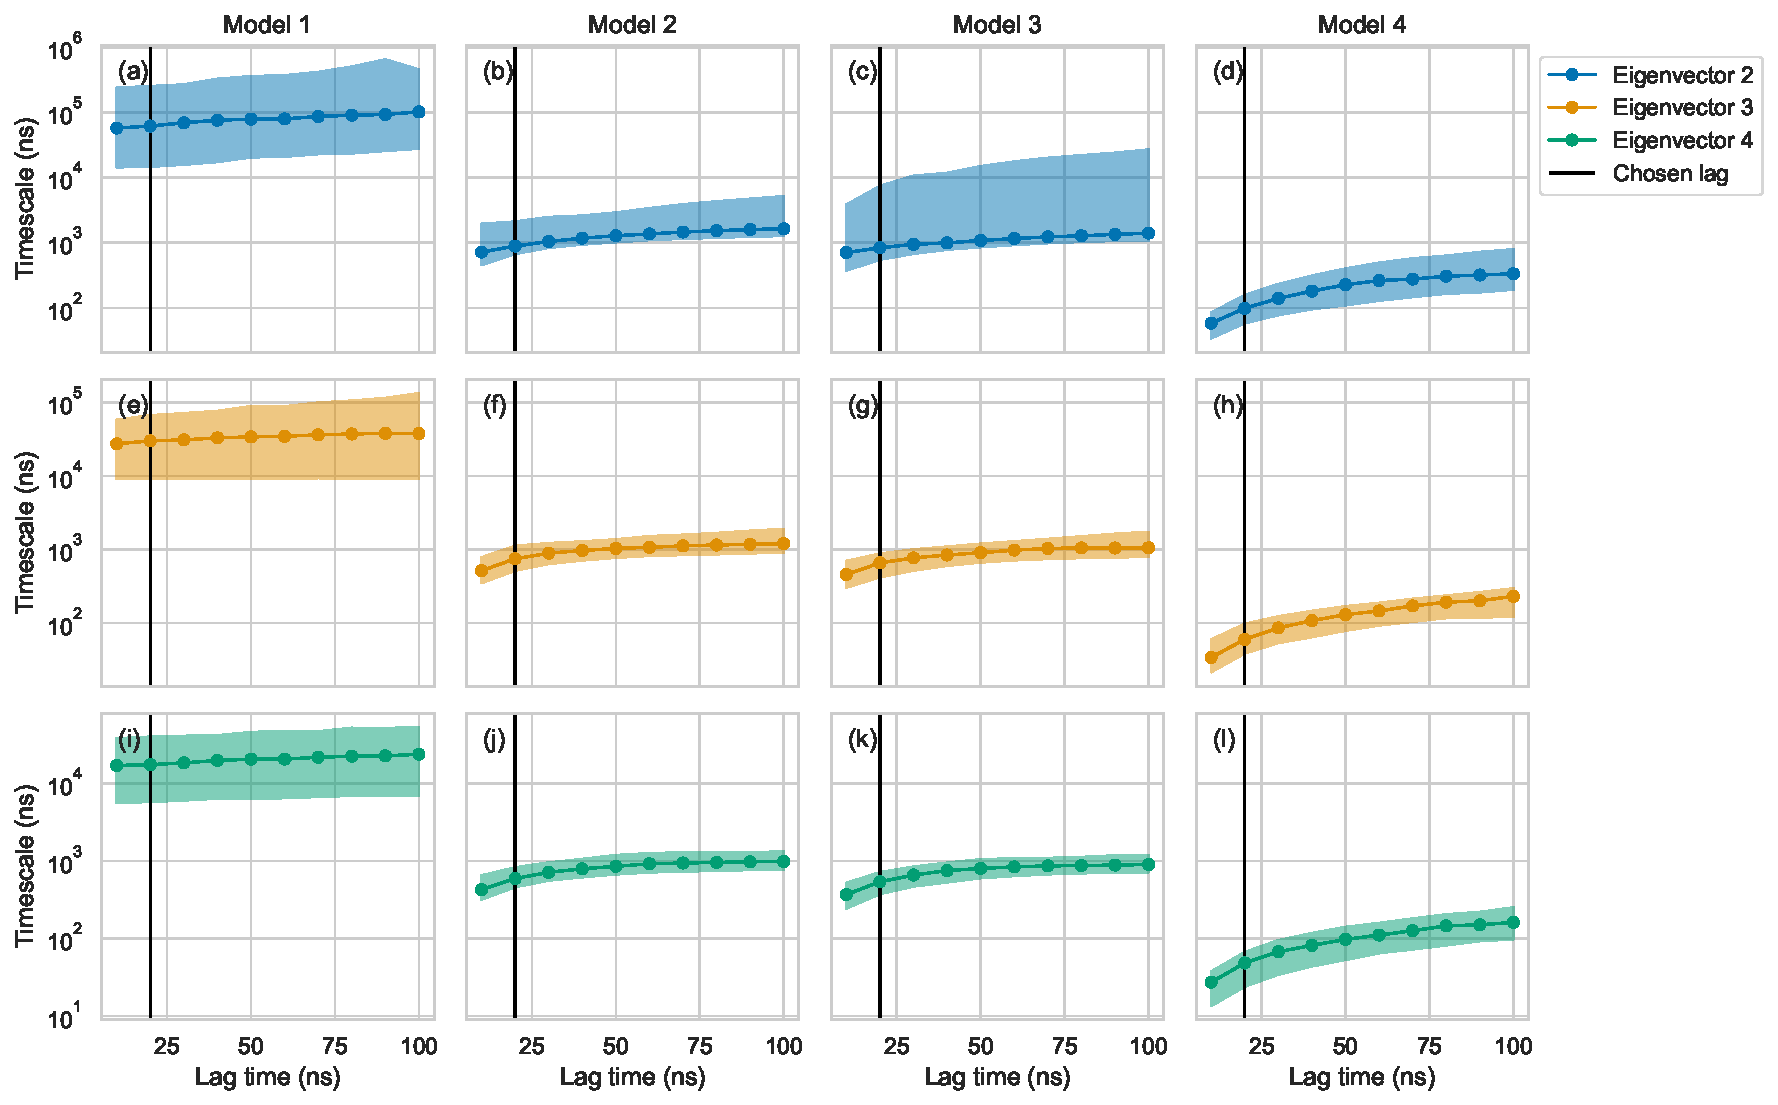
\includegraphics[width=1\textwidth]{figures/model_comparision_its/uvf.pdf}
%     \caption{\textsc{Implied timescales of homeodomain for comparator models.} Panels (a) - (d) correspond to models 1 - 4 which are specified in table \ref{tab:1fme_mod_defs}. Panels (a), (e) and (i) show the implied timescales for the 2nd, 3rd and 4th eigenvectors for model 1, which are the dominant eigenvectors identified in figure \ref{fig:count_num_proc}.  Panels (b), (f) and (j) show the implied timescales for model 2 and so on.}
%     \label{fig:uvf_its}
% \end{figure}

% \begin{figure}[h]
%     \centering
%     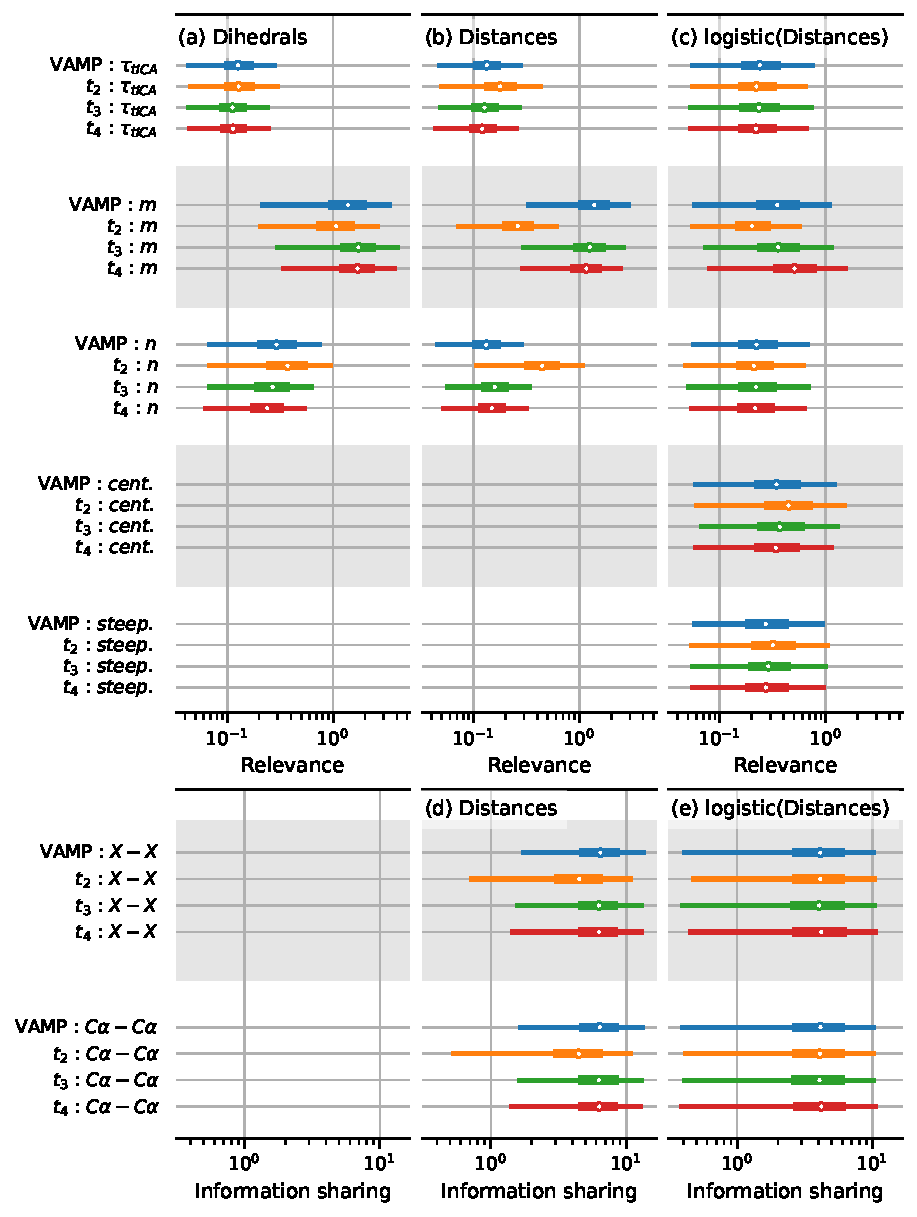
\includegraphics[height=0.8\textheight]{figures/sensitivities/uvf_sensitivity.pdf}
%     \caption{\textsc{Homeodomain hyperparameter relevance and information sharing}. Shown are the  median (white dot), \SI{50}{\percent} and \SI{95}{\percent} credible intervals (thick and thin lines respectively).  Panels (a)-(c) show the hyperparameter relevance for of each hyperparameter in determining the log of the VAMP-2 score (`VAMP' in blue) and the log of the dominant timescales ($t_{2}, t_{3}, ...$ in orange, green etc.). $\tau_{\mathrm{tICA}}$ is the TICA lag-time; $m$ is the TICA dimension, $n$ is the number of cluster centers; $cent.$ and $steep.$ are the center and steepness parameters of the logistic transform. Panels (d)-(e) show the information sharing parameters for whether the contact distances use the `closest-heavy' ($X-X$) or the `alpha-carbon' ($C_{\alpha}-C_{\alpha}$) scheme.  }
%     \label{fig:uvf_sense}
% \end{figure}







% \end{document}


